% notation for the parts and the shadow of a General Number (Chapter 3, Section 3.5)
\providecommand{\Com}{\operatorname{Com}}
\providecommand{\Sh}{\operatorname{Sh}}
%************************************************
\chapter{The Interaction Law}\label{ch:interaction}
%************************************************

\chapterlead{Mass and charge enter the General Number Plane: one number for each particle, one law for every pair of particles, a triangle that becomes a new identity card for matter, and one way of reading the law, in its own plane, in which like charges push apart with the full strength of Coulomb's law.}

\scene{London, 1849}

On 19 March 1849, Michael Faraday wrote five words in capital letters in his laboratory notebook: \enquote{ALL THIS IS A DREAM.} He had been thinking about gravity. Eighteen years earlier he had discovered that a moving magnet drives an electric current around a coil of wire, and he had spent his life finding links between powers of nature that others believed to be separate: electricity and magnetism, magnetism and light. Now he wondered whether gravity, too, was tied to electricity. If a body falling towards the Earth could stir up electricity, the two would be two faces of a single power.

The dream did not stop him. \enquote{Still examine it by a few experiments,} he went on in the same entry. \enquote{Nothing is too wonderful to be true, if it be consistent with the laws of nature; and in such things as these, experiment is the best test of such consistency.} He wound hundreds of feet of copper wire into a coil, connected it to a sensitive galvanometer, and let the coil fall again and again from a height of about eleven metres onto a cushion, watching the needle for the smallest kick (\Cref{fig:faraday-coil}).

\begin{figure}[tb]
\myfloatalign
\begin{tikzpicture}[>=Stealth, every node/.style={font=\small}]
  % ceiling and floor
  \draw[gray!55, line width=1.2pt] (-1.2,5.4) -- (2.2,5.4);
  \draw[gray!55, line width=1.2pt] (-1.2,0) -- (8.2,0);
  % height of the fall
  \draw[<->, gray] (-0.8,0.45) -- (-0.8,4.8) node[midway, left, align=right, font=\footnotesize] {about\\ eleven\\ metres};
  % the coil at the top, and a faint copy of it on the way down
  \foreach \y in {0,0.09,...,0.56} \draw[Maroon!80!black, thick] (0.4,4.25+\y) ellipse (0.42 and 0.1);
  \foreach \y in {0,0.09,...,0.56} \draw[Maroon!28] (0.4,2.15+\y) ellipse (0.42 and 0.1);
  \draw[->, thick, gray] (0.4,4.0) -- (0.4,3.0);
  \node[anchor=west, font=\footnotesize] at (0.95,4.02) {coil of copper wire};
  \node[anchor=west, font=\footnotesize, text=gray!80!black] at (0.95,2.45) {falling};
  % the cushion
  \fill[gray!20, rounded corners=3pt] (-0.3,0) rectangle (1.1,0.4);
  \draw[gray!60, rounded corners=3pt] (-0.3,0) rectangle (1.1,0.4);
  \node[anchor=west, font=\footnotesize] at (1.2,0.2) {cushion};
  % the long wires to the galvanometer
  \draw[gray!70!black] (0.82,4.82) .. controls (3.6,5.7) and (6.95,4.9) .. (6.75,1.72);
  \draw[gray!70!black] (0.82,4.3) .. controls (3.4,5.2) and (6.45,4.5) .. (6.25,1.72);
  % the galvanometer, its needle at zero
  \draw[thick, fill=white] (6.5,1.0) circle (0.78);
  \draw[gray] (6.5,1.0) ++(35:0.58) arc (35:145:0.58);
  \foreach \t in {35,62.5,90,117.5,145} \draw[gray] (6.5,1.0) ++(\t:0.58) -- ++(\t:0.1);
  \draw[very thick, RoyalBlue] (6.5,1.0) -- ++(90:0.6);
  \fill (6.5,1.0) circle (1.3pt);
  \node[font=\footnotesize, align=center] at (6.5,-0.5) {galvanometer: the needle\\ stayed at zero};
\end{tikzpicture}
\caption[Faraday's falling coil]{Faraday's test of 1849, as he described it (not to scale). A coil of copper wire falls from a height of about eleven metres onto a cushion, and long wires join it to a sensitive galvanometer. If falling under gravity stirred up electricity, the needle would kick. It stayed at zero \citep{Faraday1851}.}
\label{fig:faraday-coil}
\end{figure}
\begin{figure}[!b]
\myfloatalign
\begin{tikzpicture}[>=Stealth,
    mapstep/.style={draw=RoyalBlue!55, fill=RoyalBlue!6, rounded corners=2pt, text width=2.2cm,
                 align=flush center, inner sep=4pt, font=\footnotesize, minimum height=2.85cm, anchor=north},
    mapfeed/.style={font=\footnotesize, text=gray!75!black, align=center},
    mapflow/.style={->, thick, RoyalBlue!70}]
  \node[mapstep] (s1) at (0,0) {\textbf{1. Particles and\\ two laws}\\[1pt]
    {\color{gray!75!black}\Cref{sec:formal-definitions}}\\[5pt]
    a pair $(m, q)$;\\ Newton, Coulomb};
  \node[mapstep] (s2) at (2.85,0) {\textbf{2. One number,\\ one law}\\[1pt]
    {\color{gray!75!black}\Cref{sec:cosmic-mass}}\\[5pt]
    $\mu = m + q\Gp$;\\ three terms};
  \node[mapstep] (s3) at (5.7,0) {\textbf{3. The plane of\\ our universe}\\[1pt]
    {\color{gray!75!black}\Cref{subsec:relative-plane}}\\[5pt]
    $|\Gp| = \sqrt{K/G}$;\\ the angle $79.86^\circ$};
  \node[mapstep] (s4) at (8.55,0) {\textbf{4. A new\\ identity}\\[1pt]
    {\color{gray!75!black}\Cref{sec:identity}}\\[5pt]
    a triangle\\ $(r, \alpha, \phi)$};
  \node[mapstep] (s5) at (2.85,-3.45) {\textbf{5. Reading\\ the law}\\[1pt]
    {\color{gray!75!black}\Cref{sec:reading-law}}\\[5pt]
    the real part;\\ the hydrogen\\ test};
  \node[mapstep] (s6) at (5.7,-3.45) {\textbf{6. Like charges\\ push apart}\\[1pt]
    {\color{gray!75!black}\Cref{sec:why-mirror}}\\[5pt]
    on a line they\\ would pull; at\\ $79.86^\circ$ they push};
  \draw[mapflow] (s1.east) -- (s2.west);
  \draw[mapflow] (s2.east) -- (s3.west);
  \draw[mapflow] (s3.east) -- (s4.west);
  \draw[mapflow, rounded corners=4pt] (s4.south) -- ++(0,-0.3) -| ($(s5.north)+(0,0.3)$) -- (s5.north);
  \draw[mapflow] (s5.east) -- (s6.west);
  \node[mapfeed] (c1) at (0,1.05) {from Chapter~\ref{ch:one-number}:\\ two laws, one shape};
  \node[mapfeed] (c2) at (2.85,1.05) {from Chapter~\ref{ch:general-numbers}:\\ $z = a + b\Gp$};
  \node[mapfeed] (c4) at (8.55,1.05) {from Chapter~\ref{ch:general-numbers}:\\ numbers as triangles};
  \draw[->, gray!70] (c1.south) -- (s1.north);
  \draw[->, gray!70] (c2.south) -- (s2.north);
  \draw[->, gray!70] (c4.south) -- (s4.north);
  \node[mapfeed] (c3) at (5.7,1.05) {from Chapter~\ref{ch:general-numbers}:\\ the mirror root};
  \draw[->, gray!70] (c3.south) -- (s3.north);
  \node[mapfeed, anchor=east] (c5) at ($(s5.west)+(-0.35,0)$) {from Chapter~\ref{ch:general-numbers}:\\ the Rule\\ of the Square};
  \draw[->, gray!70] (c5.east) -- (s5.west);
  \node[mapfeed, anchor=west] (out) at ($(s6.east)+(0.5,-1.42)$) {to Chapter~\ref{ch:standard-model}:\\ the Cosmic Mass\\ Standard Model};
  \draw[->, gray!70] ($(s6.east)+(0,-1.42)$) -- (out.west);
\end{tikzpicture}
\caption[The road through the chapter]{The road through the chapter. Each box is one step, with the section where it is taken. Ideas come in from Chapters~\ref{ch:one-number} and~\ref{ch:general-numbers}, and the last step shows why like charges push apart at the angle $79.86^\circ$, on which Chapter~\ref{ch:standard-model} builds.}
\label{fig:interaction-map}
\end{figure}

The needle did not move. In his report to the Royal Society, Faraday wrote: \enquote{Here end my trials for the present. The results are negative. They do not shake my strong feeling of the existence of a relation between gravity and electricity, though they give no proof that such a relation exists} \citep{Faraday1851}.

This chapter takes up Faraday's feeling with the tools of Part~\ref{pt:beyond}. We will not drop a coil; we will look instead at the two laws themselves.

\bigskip

Physics sorts the forces of nature into four kinds: gravitational, electromagnetic, weak and strong. Two of them, gravity and electricity, are written in laws of the same shape (\Cref{fig:two-laws}). Yet one law speaks of mass and the other of charge, and a particle such as the proton carries both at once. Could the two laws be one law, read in two ways?

This chapter answers with one new object, the \textbf{Cosmic Mass}, which writes the mass and the charge of a particle as a single General Number. It is built with the \textbf{Composer Unit} $\Gp$ of Chapter~\ref{ch:general-numbers}, the second unit of a number plane whose second axis leans; for the cosmic mass that axis leans at $79.86^\circ$. One law built on cosmic masses, read in the plane in which it lives, gives back Newton's gravity and Coulomb's law, each at full strength, and its third term, the \textbf{Coupling Force}, finds its place in the Composer coordinate.

The chapter is a concrete attempt to rethink the algebraic and geometric foundation of force and of the identity of a particle, not an abstract exercise. Every formal statement is followed by plain words, and every calculation is written out step by step.

\paragraph{The road through this chapter.}
The chapter climbs in six steps, shown in \Cref{fig:interaction-map}. The first three build the cosmic mass, its law and the plane in which it lives; the fourth gives every particle a new identity card; the last two read the law in its own plane, test the reading on the hydrogen atom, and show why like charges push apart. Every step takes its mathematics from Chapter~\ref{ch:general-numbers}, and \Cref{tab:gn-tools} lists where.

%------------------------------------------------
\section{Two Numbers, Two Laws}\label{sec:formal-definitions}
%------------------------------------------------

\subsection{A Particle and Its Signature}\label{subsec:dual-scalar}

Let us begin by considering two particles labeled $P(A)$ and $P(B)$. Each particle is characterized not only by its mass and charge but by the simultaneous presence of both as essential attributes.

\begin{figure}[tb]
\myfloatalign
\begin{tikzpicture}[>=Stealth, every node/.style={font=\small}]
  \node[draw, circle, thick, fill=gray!12, minimum size=0.95cm] (A) at (0,0) {$A$};
  \node[draw, circle, thick, fill=gray!12, minimum size=0.95cm] (B) at (8,0) {$B$};
  \node[draw=gray!60, rounded corners=3pt, fill=white, inner sep=3pt, anchor=south] at (0,0.72) {$P(A) = \begin{pmatrix} m_a \\ q_a \end{pmatrix}$};
  \node[draw=gray!60, rounded corners=3pt, fill=white, inner sep=3pt, anchor=south] at (8,0.72) {$P(B) = \begin{pmatrix} m_b \\ q_b \end{pmatrix}$};
  \draw[->, very thick, RoyalBlue] (A.east) -- ++(1.6,0) node[midway, above] {$\vec{e}_r$};
  \node[font=\footnotesize, text=RoyalBlue!80!black, anchor=north] at ($(A.east)+(0.8,-0.08)$) {length $1$};
  \draw[gray, dashed] ($(A.east)+(1.7,0)$) -- (B.west);
  \draw[gray, |<->|] (0,-1.15) -- (8,-1.15) node[midway, fill=white, inner sep=2pt] {distance $r$};
\end{tikzpicture}
\caption[Two particles and their signatures]{Two particles and their signatures (Definition~\ref{def:signature} and Remark~\ref{rem:unit-direction}). Each particle carries an identity card with two lines, its mass and its charge. The arrow $\vec{e}_r$ has length one and points from $A$ to $B$; the distance between the two particles is $r$.}
\label{fig:signature}
\end{figure}

\begin{definition}[Particle Signature]\label{def:signature}
We define each particle as a column vector consisting of its mass and electric charge:
\[
P(A) = \begin{pmatrix} m_a \\ q_a \end{pmatrix}, \qquad P(B) = \begin{pmatrix} m_b \\ q_b \end{pmatrix}
\]
where:
\begin{itemize}
  \item $m_a, m_b \in \R$ are the masses in kilograms $[kg]$
  \item $q_a, q_b \in \R$ are the electric charges in Coulombs $[C]$
\end{itemize}
\end{definition}

\begin{remark}[Unit Direction Vector]\label{rem:unit-direction}
Let $\er$ be the normalized direction vector that points from particle $A$ to particle $B$. It satisfies:
\[
|\er| = 1
\]
and defines the directional component of all force vectors in the system.
\end{remark}

% keep what follows together: break the page here if fewer than 17 lines are left
\keepblock{17}
\begin{plainwords}
A particle signature is an identity card with two lines: the mass on top, the charge below. Here are three of them, with rounded values (\Cref{app:constants} gives more digits):
\begin{align*}
P(\text{electron}) &= \begin{pmatrix} 9.109 \times 10^{-31} \\ -1.602 \times 10^{-19} \end{pmatrix}, \\
P(\text{proton}) &= \begin{pmatrix} 1.673 \times 10^{-27} \\ 1.602 \times 10^{-19} \end{pmatrix}, \\
P(\text{neutron}) &= \begin{pmatrix} 1.675 \times 10^{-27} \\ 0 \end{pmatrix},
\end{align*}
with masses in kilograms and charges in coulombs. The arrow $\er$ of Remark~\ref{rem:unit-direction} has length one, so it carries only a direction: the line from $A$ to $B$ (\Cref{fig:signature}). In every force of this chapter, $\er$ says \emph{where} the force acts, and the rest of the formula says \emph{how strongly}.
\end{plainwords}

\subsection{The Laws of Newton and Coulomb}\label{subsec:classical-forces}

\begin{definition}[Newtonian Gravitation]\label{def:newton}
The gravitational force acting between two particles at a distance $r$ apart is:
\[
\vec{F}_N = G \cdot \frac{m_a m_b}{r^2} \cdot \er
\]
where $G$ is the gravitational constant.
\end{definition}

\begin{definition}[Coulomb Electrostatics]\label{def:coulomb}
The electrostatic force acting between the two charged particles is:
\[
\vec{F}_C = K \cdot \frac{q_a q_b}{r^2} \cdot \er
\]
where $K$ is the Coulomb constant.
\end{definition}

While these two laws are treated independently, the algebraic structure of their force vectors reveals a parallelism: both forces are radially directed, follow inverse-square laws, and scale with scalar products of intrinsic properties.

\begin{plainwords}
These are the two laws of \Cref{fig:two-laws}, now written in the formal language of the chapter. Two differences between them will matter in what follows. The first is size: the ratio of the two constants is $K/G \approx 1.35 \times 10^{20}$, a number that will return in \Cref{subsec:relative-plane}. The second is behaviour: two masses always pull together, while two like charges push apart (\Cref{fig:pull-push}). Both formulas are written with the same arrow $\er$; they give the line of the force and its strength, and the difference between pulling and pushing is left to the nature of each interaction. \Cref{sec:why-mirror} will show that the cosmic mass gives this difference a reason.
\end{plainwords}

\begin{figure}[tb]
\myfloatalign
\begin{tikzpicture}[>=Stealth, every node/.style={font=\small},
    mass/.style={draw, circle, fill=gray!15, minimum size=0.78cm, inner sep=0pt},
    charge/.style={draw, circle, fill=RoyalBlue!12, minimum size=0.78cm, inner sep=0pt}]
  \def\xa{2.4}
  \def\xb{7.4}
  % the common arrow of both laws
  \draw[->, thick, RoyalBlue] (\xa,1.0) -- (\xa+1.3,1.0) node[right, font=\footnotesize] {$\vec{e}_r$, from $A$ to $B$, in both laws};
  % two masses
  \node[anchor=east, font=\footnotesize, align=right] at (0.5,0) {two masses};
  \node[mass] (a1) at (\xa,0) {$m_a$};
  \node[mass] (b1) at (\xb,0) {$m_b$};
  \draw[->, very thick, gray!70!black] (a1.east) -- ++(0.8,0);
  \draw[->, very thick, gray!70!black] (b1.west) -- ++(-0.8,0);
  \node[font=\footnotesize, text=gray!70!black] at ({(\xa+\xb)/2},0) {always pull};
  % two like charges
  \node[anchor=east, font=\footnotesize, align=right] at (0.5,-1.3) {two like\\ charges};
  \node[charge] (a2) at (\xa,-1.3) {$+$};
  \node[charge] (b2) at (\xb,-1.3) {$+$};
  \draw[->, very thick, RoyalBlue] (a2.west) -- ++(-0.8,0);
  \draw[->, very thick, RoyalBlue] (b2.east) -- ++(0.8,0);
  \node[font=\footnotesize, text=RoyalBlue] at ({(\xa+\xb)/2},-1.3) {push apart};
  % unlike charges
  \node[anchor=east, font=\footnotesize, align=right] at (0.5,-2.6) {unlike\\ charges};
  \node[charge] (a3) at (\xa,-2.6) {$+$};
  \node[charge] (b3) at (\xb,-2.6) {$-$};
  \draw[->, very thick, RoyalBlue] (a3.east) -- ++(0.8,0);
  \draw[->, very thick, RoyalBlue] (b3.west) -- ++(-0.8,0);
  \node[font=\footnotesize, text=RoyalBlue] at ({(\xa+\xb)/2},-2.6) {pull together};
\end{tikzpicture}
\caption[Pull and push]{Pull and push. Two masses always pull together. Two like charges push apart, and unlike charges pull together. Definitions~\ref{def:newton} and~\ref{def:coulomb} write both laws along the same arrow $\vec{e}_r$, and leave the direction of each force to the nature of the interaction.}
\label{fig:pull-push}
\end{figure}

%------------------------------------------------
\section{One Number, One Law}\label{sec:cosmic-mass}
%------------------------------------------------

\subsection{The Cosmic Mass}\label{subsec:cosmic-mass-def}

\begin{definition}[Cosmic Mass]\label{def:cosmic-mass}
The Cosmic Mass of a particle is defined as:
\[
\mu = m + q \cdot \Gp
\]
This scalar belongs to the General Number Plane $\GN$ and has physical units of $[kg]$, where:
\begin{itemize}
  \item $m \in \R$: classical mass
  \item $q \in \R$: electric charge
  \item $\Gp$: Composer Unit with unit $\left[\frac{kg}{C}\right]$
\end{itemize}
\end{definition}

This unified representation binds the two classical quantities, mass and charge, into a single mathematical object. This enables a single formulation for what were previously two separate physical laws.

\begin{plainwords}
The Cosmic Mass is a General Number in the sense of Definition~\ref{def:gn-parts}. Its real part is the mass, $\Re(\mu) = m$, measured along the real axis, which this chapter therefore calls the \emph{mass axis}. Its Composer coordinate is the charge $q$, and its Composer part, $\Com(\mu) = q\Gp$, is $q$ steps of the Composer Unit along the Composer axis, which carries charge (\Cref{fig:cosmic-mass-plane}). We call $m$ the \emph{mass part} and $q\Gp$ the \emph{charge part} of the cosmic mass. A neutral body has no Composer part, so its cosmic mass is a real number, $\mu = m$; a charge without mass would be a pure Composer number (Remark~\ref{rem:gn-kinds}).

The units work out just as they should. A charge in coulombs times a Composer Unit in kilograms per coulomb gives kilograms, $[C] \cdot [kg/C] = [kg]$, so both parts of $\mu$ are measured in kilograms. That is why the Cosmic Mass can be called a mass.
\end{plainwords}

From here on, every word of Chapter~\ref{ch:general-numbers} has a physical name, and \Cref{tab:dictionary} sets the two vocabularies side by side.

\begin{table}[tb]
\myfloatalign
\footnotesize
\begin{tabularx}{\textwidth}{@{}>{\raggedright\arraybackslash}p{0.43\textwidth} c >{\raggedright\arraybackslash}X@{}}
\toprule
\tableheadline{Chapter 4: mathematics} & & \tableheadline{Chapters 6 to 9: physics} \\
\midrule
General Number $z = a + b\Gp$ & \ref{def:gn-parts} & cosmic mass $\mu = m + q\Gp$ \\
real axis; Composer axis & \ref{ax:gn} & mass axis; Composer axis, or charge axis \\
real part $\Re(z) = a$ & \ref{def:gn-parts} & mass $m$, the mass part \\
Composer coordinate $b$ & \ref{def:gn-parts} & charge $q$ \\
Composer part $\Com(z) = b\Gp$ & \ref{def:gn-parts} & charge part $q\Gp$, in kilograms \\
length $\Ap$ of the Composer Unit & \ref{ax:gn} & size $\sqrt{K/G}$, read as the length $1.16043$ \\
real number; pure Composer number & \ref{rem:gn-kinds} & neutral body; a charge without mass \\
real term; cross term; square term & \ref{prop:three-terms} & gravity; Coupling Force; Coulomb's force \\
real part of a product & \ref{prop:un-real-product} & every measured force, energy and momentum (Definitions~\ref{def:reading} and~\ref{def:un-reading}) \\
Rule of the Square, $\Re(\Gp^2) = -|\Gp|^2$ & \ref{prop:square-rule} & the minus sign between gravity and Coulomb's force \\
shadow on the real axis & \ref{def:shadow} & not used to read forces \\
mirror root & \ref{thm:two-roots} & the angle $79.86^\circ$ of the Composer axis \\
backward band, $\pi/4 < \pb < 3\pi/4$ & \ref{thm:square-band} & $\Gp^2$ points back along the mass axis: like charges push \\
magnitude $M$; angles $\alpha$ and $\phi$ & \ref{def:general-polar} & cosmic magnitude $r$; charge and mass phase angles \\
ratio of the two parts, $\eta = \Ap\,b/a$ & \ref{thm:phase} & $\eta = \Gp\,q/m$ \\
equal parts, $\eta = 1$ & \ref{rem:special-triangles} & equal parts; the balanced body \\
angle $\delta$ from the Composer axis & \ref{prop:near-axis} & the lean of a charged body \\
ellipse of one magnitude & \ref{thm:ellipse} & cosmic mass ellipse \\
rings and rays & \ref{def:rings-rays} & Cosmic Mass Frame \\
sum, part by part & \ref{def:gn-product} & fusion: the charges add, the masses add less the loss \\
\bottomrule
\end{tabularx}
\caption[One object, two vocabularies]{One object, two vocabularies. On the left, the words of Chapter~\ref{ch:general-numbers}, with the number of the statement that defines each one; on the right, the names they take for the cosmic mass in Chapters~\ref{ch:interaction} to~\ref{ch:unified}.}
\label{tab:dictionary}
\end{table}

\begin{figure}[tb]
\myfloatalign
\begin{tikzpicture}[>=Stealth, scale=1.05, every node/.style={font=\small}]
  \def\ang{35}
  \begin{scope}
    \clip (-0.4,-0.6) rectangle (7.2,3.3);
    \foreach \a in {-2,...,7} \draw[gray!22] ($(\a,0)+(\ang:-2)$) -- ($(\a,0)+(\ang:6)$);
    \foreach \b in {-1,...,5} \draw[gray!22] ($(-2,0)+(\ang:{\b*0.75})$) -- ($(8,0)+(\ang:{\b*0.75})$);
  \end{scope}
  \draw[->, gray] (-0.4,0) -- (7.2,0) node[below left] {real axis: mass};
  \draw[->, gray] (0,0) -- (\ang:4.9) node[above] {Composer axis: charge};
  \draw[->, very thick, Maroon] (0,0) -- (3,0) node[midway, below] {$m$};
  \draw[->, very thick, RoyalBlue] (3,0) -- ($(3,0)+(\ang:2.25)$) node[midway, below right] {$q \cdot \mathcal{G}_{\bar{\phi}}$};
  \draw[->, very thick] (0,0) -- ($(3,0)+(\ang:2.25)$);
  \fill ($(3,0)+(\ang:2.25)$) circle (1.6pt) node[above right] {$\mu = m + q \cdot \mathcal{G}_{\bar{\phi}}$};
  \draw[gray] (0.8,0) arc (0:\ang:0.8);
  \node[gray] at ({\ang/2}:1.1) {$\bar{\phi}$};
  \fill (0,0) circle (1.2pt) node[below left] {$0$};
\end{tikzpicture}
\caption[The cosmic mass of a particle]{The cosmic mass of a particle as a General Number (Definition~\ref{def:cosmic-mass}): $m$ steps along the real axis, which carries mass, and $q$ steps of the Composer Unit along the Composer axis, which carries charge. The angle $\bar{\phi}$ is drawn at $35^\circ$ and the two parts with comparable lengths, so that the construction is easy to see; \Cref{subsec:relative-plane} finds the angle of our universe.}
\label{fig:cosmic-mass-plane}
\end{figure}

\subsection{The Cosmic Interaction Law}\label{subsec:cosmic-force}

\begin{theorem}[Cosmic Interaction Law]\label{thm:cosmic-law}
Let $\mu_a = m_a + q_a\Gp$ and $\mu_b = m_b + q_b\Gp$ be the Cosmic Masses of particles $A$ and $B$. Then the total interaction force is given by:
\[
\vec{F}_G = G \cdot \frac{\mu_a \mu_b}{r^2} \cdot \er
\]
Expanding this, we obtain:
\begin{align*}
\vec{F}_G &= G \cdot \frac{m_a m_b}{r^2} \cdot \er \\
          &\quad + \Gp^2 \cdot G \cdot \frac{q_a q_b}{r^2} \cdot \er \\
          &\quad + \Gp \cdot G \cdot \frac{m_a q_b + q_a m_b}{r^2} \cdot \er
\end{align*}
\end{theorem}

% keep what follows together: break the page here if fewer than 11 lines are left
\keepblock{11}
\begin{plainwords}
The law has exactly the shape of Newton's law, with cosmic masses in place of masses. Its three lines are the three terms of a product of two General Numbers (Proposition~\ref{prop:three-terms}): the real term gives gravity, the cross term the Coupling Force and the square term the Coulomb-like force (\Cref{fig:product-area}):
\[
(m_a + q_a\Gp)(m_b + q_b\Gp) = m_a m_b + (m_a q_b + q_a m_b)\,\Gp + q_a q_b\,\Gp^2 .
\]
\end{plainwords}

\begin{figure}[tb]
\myfloatalign
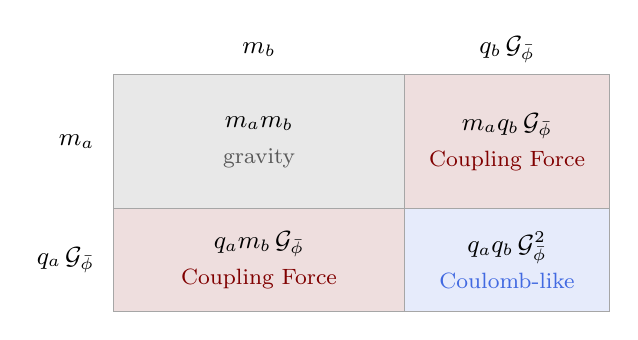
\begin{tikzpicture}[every node/.style={font=\small}]
  \def\wa{3.7}
  \def\wb{2.6}
  \def\ha{1.7}
  \def\hb{1.3}
  \fill[gray!18] (0,0) rectangle (\wa,\ha);
  \fill[Maroon!13] (\wa,0) rectangle ({\wa+\wb},\ha);
  \fill[Maroon!13] (0,-\hb) rectangle (\wa,0);
  \fill[RoyalBlue!13] (\wa,-\hb) rectangle ({\wa+\wb},0);
  \draw[gray!70] (0,-\hb) rectangle ({\wa+\wb},\ha);
  \draw[gray!70] (\wa,-\hb) -- (\wa,\ha);
  \draw[gray!70] (0,0) -- ({\wa+\wb},0);
  % the two brackets along the edges
  \node at ({\wa/2},{\ha+0.32}) {$m_b$};
  \node at ({\wa+\wb/2},{\ha+0.32}) {$q_b\,\mathcal{G}_{\bar{\phi}}$};
  \node[anchor=east] at (-0.12,{\ha/2}) {$m_a$};
  \node[anchor=east] at (-0.12,{-\hb/2}) {$q_a\,\mathcal{G}_{\bar{\phi}}$};
  % the four pieces
  \node[align=center] at ({\wa/2},{\ha/2}) {$m_a m_b$\\[2pt] {\footnotesize\color{gray!70!black} gravity}};
  \node[align=center] at ({\wa+\wb/2},{\ha/2}) {$m_a q_b\,\mathcal{G}_{\bar{\phi}}$\\[2pt] {\footnotesize\color{Maroon} Coupling Force}};
  \node[align=center] at ({\wa/2},{-\hb/2}) {$q_a m_b\,\mathcal{G}_{\bar{\phi}}$\\[2pt] {\footnotesize\color{Maroon} Coupling Force}};
  \node[align=center] at ({\wa+\wb/2},{-\hb/2}) {$q_a q_b\,\mathcal{G}_{\bar{\phi}}^2$\\[2pt] {\footnotesize\color{RoyalBlue} Coulomb-like}};
\end{tikzpicture}
\caption[Multiplying out the two brackets]{Multiplying out the two brackets, as at school (\Cref{thm:cosmic-law} and Proposition~\ref{prop:three-terms}). The product $(m_a + q_a\mathcal{G}_{\bar{\phi}})(m_b + q_b\mathcal{G}_{\bar{\phi}})$ is the area of the whole rectangle. Mass times mass gives gravity (grey), charge times charge gives the Coulomb-like term with $\mathcal{G}_{\bar{\phi}}^2$ (blue), and the two cross products, each mass with the other particle's charge, give the Coupling Force (red). The pieces are not drawn to scale.}
\label{fig:product-area}
\end{figure}

\begin{remark}\label{rem:three-components}
The force decomposes naturally into three components:
\begin{itemize}
  \item Gravitational force (mass-mass)
  \item Coulomb-like force (charge-charge), scaled by $\Gp^2$
  \item A novel cross-coupling term (mass-charge), scaled by $\Gp$
\end{itemize}
This third term introduces a possible new fundamental interaction, which we call the \textbf{Coupling Force}.
\end{remark}

\begin{figure}[tb]
\myfloatalign
\begin{tikzpicture}[>=Stealth, every node/.style={font=\small}]
  % the two particles
  \draw[rounded corners=6pt, thick, gray] (-0.75,-1.6) rectangle (0.75,1.6);
  \draw[rounded corners=6pt, thick, gray] (6.25,-1.6) rectangle (7.75,1.6);
  \node[gray] at (0,2.0) {particle $A$};
  \node[gray] at (7,2.0) {particle $B$};
  \node[draw, circle, fill=gray!15, minimum size=0.95cm] (ma) at (0,0.8) {$m_a$};
  \node[draw, circle, fill=RoyalBlue!12, minimum size=0.95cm] (qa) at (0,-0.8) {$q_a$};
  \node[draw, circle, fill=gray!15, minimum size=0.95cm] (mb) at (7,0.8) {$m_b$};
  \node[draw, circle, fill=RoyalBlue!12, minimum size=0.95cm] (qb) at (7,-0.8) {$q_b$};
  % the three components
  \draw[very thick, gray!70!black] (ma) -- (mb) node[midway, above] {gravitational: $G$};
  \draw[very thick, RoyalBlue] (qa) -- (qb) node[midway, below] {Coulomb-like: $\mathcal{G}_{\bar{\phi}}^2 \cdot G$};
  \draw[very thick, Maroon, dashed] (ma) -- (qb);
  \draw[very thick, Maroon, dashed] (qa) -- (mb);
  \node[fill=white, inner sep=2pt, text=Maroon, align=center] at (3.5,0) {Coupling Force:\\ $\mathcal{G}_{\bar{\phi}} \cdot G$};
\end{tikzpicture}
\caption[Three components of one law]{Three components of one law (Theorem~\ref{thm:cosmic-law} and Remark~\ref{rem:three-components}). Each pairing has its own constant: $G$ for mass with mass, $\mathcal{G}_{\bar{\phi}}^2 \cdot G$ for charge with charge, and $\mathcal{G}_{\bar{\phi}} \cdot G$ for each mass with the other particle's charge.}
\label{fig:three-components}
\end{figure}

% keep what follows together: break the page here if fewer than 9 lines are left
\keepblock{9}
\begin{plainwords}
Three things can be read straight off the law.
\begin{itemize}
  \item For two neutral particles, $q_a = q_b = 0$, the second and third lines vanish and only Newton's gravity is left. Nothing changes for uncharged matter.
  \item The Coupling Force vanishes whenever $m_a q_b + q_a m_b = 0$. For example, between a particle and its antiparticle, which have the same mass and opposite charges, the Coupling Force is exactly zero. (The Composer coordinate of their product, found in \Cref{subsec:law-read}, is still not zero: it also holds a share of the term of two charges.)
  \item The second line looks like Coulomb's law, with $\Gp^2 \cdot G$ in the place of $K$. The next section asks what the Composer Unit must be for the two to agree.
\end{itemize}
\end{plainwords}

%------------------------------------------------
\section{The Relative Plane of Our Universe}\label{subsec:relative-plane}
%------------------------------------------------

The Composer Unit has a size and an angle. This section finds both from the constants of nature, first the size and then the angle (\Cref{fig:constants-angle}).

\begin{figure}[tb]
\myfloatalign
\begin{tikzpicture}[>=Stealth,
    mapstep/.style={draw=RoyalBlue!55, fill=RoyalBlue!6, rounded corners=2pt, text width=2.4cm,
                 align=flush center, inner sep=4pt, font=\footnotesize, minimum height=2.85cm, anchor=north},
    mapfeed/.style={font=\footnotesize, text=gray!75!black, align=center},
    mapflow/.style={->, thick, RoyalBlue!70}]
  \node[mapstep] (s1) at (0,0) {\textbf{1. The\\ constants}\\[1pt]
    {\color{gray!75!black}\Cref{subsec:relative-plane}}\\[5pt]
    $G$ and $K$, so\\ $K/G \approx$\\ $1.3466 \times 10^{20}$};
  \node[mapstep] (s2) at (2.95,0) {\textbf{2. The size of\\ the unit}\\[1pt]
    {\color{gray!75!black}Remark~\ref{rem:light}}\\[5pt]
    $\mathcal{G}_{\bar{\phi}} = \sqrt{K/G}$\\ \mbox{$\approx 1.16043 \times 10^{10}$}};
  \node[mapstep] (s3) at (5.9,0) {\textbf{3. The\\ split}\\[1pt]
    {\color{gray!75!black}Remark~\ref{rem:angle-value}}\\[5pt]
    length $1.16043$,\\ arrow length\\ $|\vec{u}_{\bar{\phi}}| = 10^{10}$};
  \node[mapstep] (s4) at (8.85,0) {\textbf{4. The\\ angle}\\[1pt]
    {\color{gray!75!black}Remarks~\ref{rem:angle-expressions}, \ref{rem:angle-value}}\\[5pt]
    $\bar{\phi} \approx 79.86^\circ$,\\ where like\\ charges push};
  \draw[mapflow] (s1.east) -- (s2.west);
  \draw[mapflow] (s2.east) -- (s3.west);
  \draw[mapflow] (s3.east) -- (s4.west);
  \node[mapfeed] (c3) at (5.9,1.05) {from Chapter~\ref{ch:general-numbers}:\\ a length up to $\sqrt{2}$};
  \draw[->, gray!70] (c3.south) -- (s3.north);
  \node[mapfeed] (c4) at (8.85,1.05) {from Chapter~\ref{ch:general-numbers}:\\ the mirror root};
  \draw[->, gray!70] (c4.south) -- (s4.north);
  \node[mapfeed, anchor=north] (out) at ($(s4.south)+(0,-0.4)$) {stage 2: every\\ cosmic mass is\\ written in this plane};
  \draw[->, gray!70] (s4.south) -- (out.north);
\end{tikzpicture}
\caption[From the constants of nature to the angle]{From the constants of nature to the angle of the Composer axis (stage~1 of \Cref{subsec:relative-plane}). The constants $G$ and $K$ fix the size of the Composer Unit in kilograms per coulomb. Remark~\ref{rem:angle-value} splits that size into a length and a power of ten, and Remark~\ref{rem:angle-expressions} turns the length into an angle. The book takes the mirror root of \Cref{thm:two-roots}, $79.86^\circ$, the angle at which like charges push apart (\Cref{subsec:which-root}). Every later calculation is done in the relative plane with that angle (stage~2).}
\label{fig:constants-angle}
\end{figure}

\subsection{The Size of the Composer Unit}\label{subsec:cu-size}

To determine the projection angle $\pb$, we propose using the well-known numerical values of the two universal constants:
\begin{align*}
G &= 6.67430 \times 10^{-11} \quad (\mathrm{Nm^2Kg^{-2}}), \\
K &= 8.98755 \times 10^{9} \quad (\mathrm{Nm^2C^{-2}})
\end{align*}
By imposing that the coefficient of the Coulomb force term in the expanded Cosmic Force equation matches the Coulomb constant, i.e.,
\begin{align*}
\Gp^2 \cdot G = K \Longrightarrow \Gp^2 &= \frac{K}{G} \quad (\mathrm{Kg^2C^{-2}}) \quad , \\
\Gp &= \sqrt{\frac{K}{G}} \quad (\mathrm{KgC^{-1}}) \\[6pt]
\Gp^2 &= 1.3466 \times 10^{20} \quad (\mathrm{Kg^2C^{-2}}) \quad , \\
\Gp &= 1.16043 \times 10^{10} \quad (\mathrm{KgC^{-1}})
\end{align*}
In words: the Composer Unit is about $1.16043 \times 10^{10}$ kilograms per coulomb in size. The box below checks the arithmetic, and Remark~\ref{rem:light} shows what this size is made of.

\begin{workedexample}[Worked example: checking the numbers]
Divide the two constants: $K/G = (8.98755 \times 10^{9}) / (6.67430 \times 10^{-11}) \approx 1.3466 \times 10^{20}$. Its square root is $\sqrt{1.3466 \times 10^{20}} \approx 1.16043 \times 10^{10}$. The units follow the same division: newton square metres per coulomb squared, divided by newton square metres per kilogram squared, leave kilograms squared per coulomb squared, and the square root leaves kilograms per coulomb, the unit that Definition~\ref{def:cosmic-mass} gives to the Composer Unit.
\end{workedexample}

\begin{remark}[Simplified Composer Unit Expression]\label{rem:light}
\[
\Gp = c\sqrt{\frac{\mu_0}{4\pi G}},
\]
making the speed of light $c$ a direct factor in the Composer Unit amplitude.

This form further emphasizes the connection between electromagnetic constants and gravitational constant $G$ in setting the geometry of the General Number Plane.
\end{remark}

\begin{plainwords}
Why does the speed of light appear? In the international system of units, the Coulomb constant can be written $K = \mu_0 c^2/(4\pi)$, where $\mu_0$ is the magnetic constant and $c$ the speed of light. Put this into $\Gp = \sqrt{K/G}$, and the square root splits into $c\sqrt{\mu_0/(4\pi G)}$.

That the speed of light hides inside the electric constants was one of the great surprises of the nineteenth century. In 1856 Wilhelm Weber and Rudolf Kohlrausch compared two ways of measuring the same electric charge and found that the ratio between them was a speed. Maxwell noticed that, in his units, it came out almost exactly equal to the speed of light, and concluded that light is an electromagnetic wave \citep{Maxwell1865}.
\end{plainwords}

\begin{workedexample}[Worked example: the two parts of a cosmic mass]
How large is each part of a real particle's cosmic mass? Take the electron, with $m = 9.109 \times 10^{-31}$ kg and $q = -1.602 \times 10^{-19}$ C. With the size of the Composer Unit found above, $1.16043 \times 10^{10}$ kg/C, the charge part has size
\[
|q| \times 1.16043 \times 10^{10} \approx 1.859 \times 10^{-9} \text{ kg}.
\]
The charge part is about $2 \times 10^{21}$ times larger than the mass part. For the proton, the same calculation gives a ratio of about $1.1 \times 10^{18}$. Square that ratio and you get about $1.2 \times 10^{36}$: the factor by which the electric push between two protons beats their gravitational pull, the number we met in Chapter~\ref{ch:one-number}. This is no accident. The condition $\Gp^2 \cdot G = K$ was chosen precisely so that, inside the Cosmic Interaction Law, the charge part of a cosmic mass weighs as much as the charge does in Coulomb's law.

\Cref{fig:two-parts} draws these sizes on a scale of powers of ten, together with the three terms of \Cref{thm:cosmic-law} for two protons one metre apart. Read as ordinary forces along $\er$, the gravitational term is about $1.9 \times 10^{-64}$ newtons, the Coulomb-like term about $2.3 \times 10^{-28}$ newtons, and the Coupling Force about $4.2 \times 10^{-46}$ newtons. The Coupling Force sits halfway between the other two, up to a factor of two, because its coefficient is the geometric mean of the two constants: $\Gp \cdot G = \sqrt{K/G} \cdot G = \sqrt{KG}$. How the three terms combine into one measured force is the subject of \Cref{subsec:reading}.
\end{workedexample}

\begin{figure}[tb]
\myfloatalign
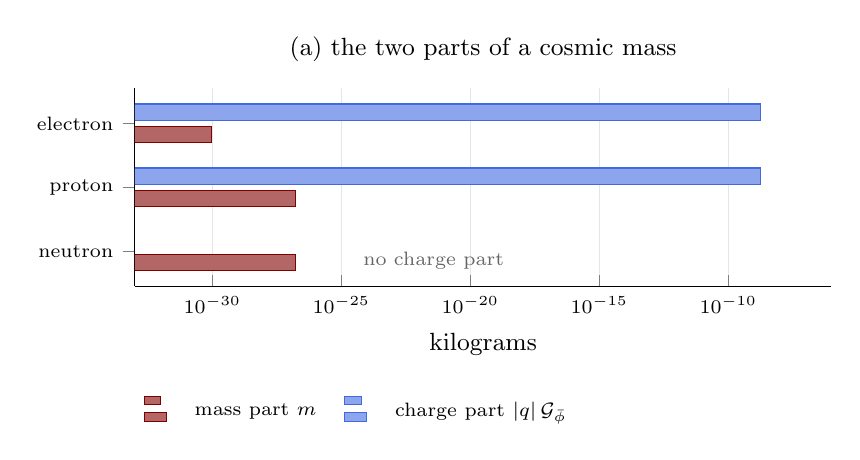
\begin{tikzpicture}
  \begin{axis}[
    xbar, xmode=log, log origin=infty,
    width=0.86\textwidth, height=4.1cm,
    xmin=1e-33, xmax=1e-6,
    xtick={1e-30,1e-25,1e-20,1e-15,1e-10},
    ytick={1,2,3}, yticklabels={neutron, proton, electron},
    ymin=0.45, ymax=3.55, bar width=6pt,
    xlabel={kilograms},
    axis lines*=left, xmajorgrids, grid style={gray!20},
    tick label style={font=\scriptsize}, label style={font=\small},
    title={(a) the two parts of a cosmic mass}, title style={font=\small},
    legend style={font=\scriptsize, draw=none, fill=none, at={(0.0,-0.52)}, anchor=north west, legend columns=2, column sep=8pt},
    legend cell align=left]
    \addplot[fill=Maroon!60, draw=Maroon] coordinates {(1.675e-27,1) (1.673e-27,2) (9.109e-31,3)};
    \addplot[fill=RoyalBlue!60, draw=RoyalBlue] coordinates {(1.859e-9,2) (1.859e-9,3)};
    \legend{mass part $m$, charge part $|q|\,\mathcal{G}_{\bar{\phi}}$}
    \node[font=\scriptsize, text=gray!80!black, anchor=west] at (axis cs:3e-25,0.85) {no charge part};
  \end{axis}
\end{tikzpicture}

\bigskip
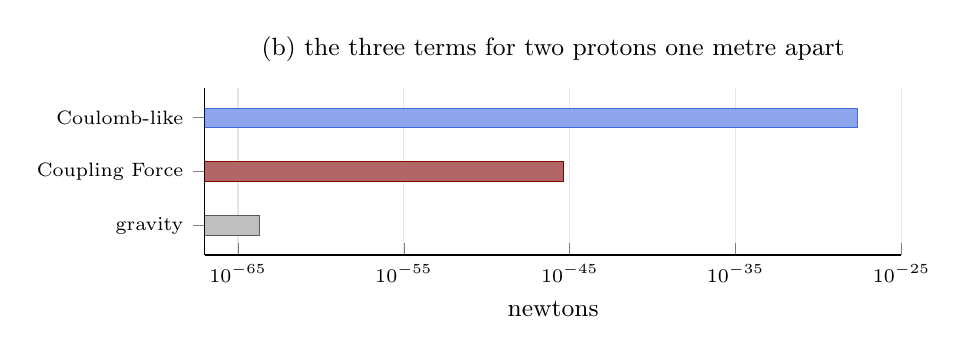
\begin{tikzpicture}
  \begin{axis}[
    xbar, xmode=log, log origin=infty,
    width=0.86\textwidth, height=3.7cm,
    xmin=1e-67, xmax=1e-25,
    xtick={1e-65,1e-55,1e-45,1e-35,1e-25},
    ytick={1,2,3}, yticklabels={gravity, Coupling Force, Coulomb-like},
    ymin=0.45, ymax=3.55, bar width=7pt, bar shift=0pt,
    xlabel={newtons},
    axis lines*=left, xmajorgrids, grid style={gray!20},
    tick label style={font=\scriptsize}, label style={font=\small},
    title={(b) the three terms for two protons one metre apart}, title style={font=\small}]
    \addplot[fill=gray!50, draw=gray!70!black] coordinates {(1.868e-64,1)};
    \addplot[fill=Maroon!60, draw=Maroon] coordinates {(4.152e-46,2)};
    \addplot[fill=RoyalBlue!60, draw=RoyalBlue] coordinates {(2.307e-28,3)};
  \end{axis}
\end{tikzpicture}
\caption[Sizes on a scale of powers of ten]{Sizes on a scale of powers of ten. (a) The two parts of the cosmic masses of the electron, the proton and the neutron, in kilograms. The charge part $|q|\,\mathcal{G}_{\bar{\phi}} \approx 1.859 \times 10^{-9}$ kg is the same for the electron and the proton, and the neutron has none. (b) The three terms of \Cref{thm:cosmic-law} for two protons one metre apart, in newtons, if each is read as an ordinary force along $\vec{e}_r$. The Coupling Force sits halfway between gravity and the Coulomb-like term, up to a factor of two.}
\label{fig:two-parts}
\end{figure}

\subsection{From the Size to an Angle}\label{subsec:cu-angle}

The Composer Unit is not a universal constant but rather a pa\-ram\-e\-trized unit whose behavior depends on a geometric angle $\pb$. As $\pb$ varies from $0$ to $\pi$, the amplitude $\Ap = \left|\sqrt{2}\sin\left(\pb + \frac{\pi}{4}\right)\right|$ varies between $0$ and $\sqrt{2}$, modulating both the scalar strength and directional behavior of the Composer axis.

\begin{remark}[Expressions for the Projection Angle $\pb$]\label{rem:angle-expressions}
Based on the amplitude definitions of the Composer Unit $\Gp$ and its square $\Gp^2$, we can express the projection angle $\pb$ as follows:
\[
\pb = \arcsin\left(\frac{\Gp}{\sqrt{2}}\right) - \frac{\pi}{4}, \qquad \text{and} \qquad \pb = \frac{1}{2}\arcsin\left(\Gp^2 - 1\right).
\]
These inverse relations enable solving for $\pb$ given the amplitude values of $\Gp$ or $\Gp^2$, facilitating the determination of the Subgeneral Plane configuration.
\end{remark}

% keep what follows together: break the page here if fewer than 5 lines are left
\keepblock{5}
\begin{plainwords}
These are the formulas of \Cref{thm:two-roots}, written with the symbol $\Gp$ for the length of the Composer Unit. Each turns a length into an angle.
\end{plainwords}


\begin{remark}[Numerical Value of the Projection Angle $\pb$]\label{rem:angle-value}
Using the physical constants to determine the Composer Unit modulus and considering the direction vector magnitude as
\[
|\up| = 10^{10},
\]
we obtained the normalized Composer Unit value:
\[
\Gp \approx 1.16043 \cdot \up .
\]
Applying the formula
\[
\pb = \arcsin\left(\frac{1.16043}{\sqrt{2}}\right) - \frac{\pi}{4},
\]
we calculate the projection angle to be
\[
\pb \approx 0.1770 \text{ radians} \approx 10.14^\circ .
\]
This value of $\pb$ defines the specific skew angle of the Composer axis relative to the real axis for the physical universe modeled within the General Number Plane framework. It quantifies the departure from orthogonality and sets the geometric basis for unifying gravitational and electromagnetic interactions.
\end{remark}

\begin{plainwords}
Remark~\ref{rem:angle-value} splits the size of the Composer Unit, $1.16043 \times 10^{10}$, into two factors. The power of ten becomes the length of the direction arrow, $|\up| = 10^{10}$, and the number $1.16043$ is read as the length $\Ap$ of the Composer Unit, which Axiom~\ref{ax:gn} calls its amplitude. The number fits that role, since the length lies between $0$ and $\sqrt{2} \approx 1.414$ (\Cref{fig:amplitude}). The formula of Remark~\ref{rem:angle-expressions} then turns the length into an angle: $1.16043/\sqrt{2} \approx 0.82055$, its arcsine is about $55.14^\circ$, and taking away $45^\circ$ leaves $10.14^\circ$.
\end{plainwords}

The same length belongs to a second angle. By \Cref{thm:two-roots}, a length between $1$ and $\sqrt{2}$ is reached at two angles, mirror images of each other about $45^\circ$, and the arcsine button of a calculator returns only the first. The second, the mirror root, is
\[
\pb = \frac{\pi}{2} - 0.1770 \approx 1.3938 \text{ radians} \approx 79.86^\circ ,
\]
and it is the angle of the Composer axis in this book, from here to the last page.

The book takes this angle because it shows why like charges push apart and do not pull. The term of two charges in the law of \Cref{thm:cosmic-law} carries the square $\Gp^2$ (Remark~\ref{rem:three-components}), and the square leans at twice the angle of the Composer Unit (\Cref{thm:powers}). At $79.86^\circ$ it leans at $159.72^\circ$: past the upright, pointing backward, against the mass axis along which two masses pull. This is the backward band of \Cref{thm:square-band}, and the mirror root lies inside it (Corollary~\ref{cor:roots-band}). So in this plane the arrow of two like charges points against the arrow of two masses: where masses pull, like charges push. \Cref{subsec:which-root} checks this with both readings of the law.

Once the angle $\pb$ is set, all future computations of the General scalar
\[
\mu = m + q\Gp
\]
and cosmic interactions are carried out within this fixed Relative Plane.

In summary, the characterization of the General Number Plane occurs in two stages:
\begin{enumerate}
  \item \textbf{Angle Selection:} Compute or assume a specific $\pb$ based on physical constants or modeling choices.
  \item \textbf{Activation:} Use $\Gp$ as the base Composer Unit in all scalar-vector definitions and operations.
\end{enumerate}

% keep what follows together: break the page here if fewer than 7 lines are left
\keepblock{7}
\begin{plainwords}
Remember the fan of relative planes in \Cref{fig:fan}: each blade is a Composer axis at its own angle, with its own length. The General Number Plane is the whole fan, but a physical theory must work in one blade, and the two stages above choose it (\Cref{fig:constants-angle}): the blade at $79.86^\circ$, sized by the constants of nature.
\end{plainwords}

%------------------------------------------------
\section{A New Identity Card for Particles}\label{sec:identity}
%------------------------------------------------

In the relative plane, every particle is one point: the tip of its cosmic mass, reached by walking the mass along the mass axis and then the charge part along the Composer axis (\Cref{fig:cosmic-mass-plane}). The five remarks of this section describe that point with one length and two angles, as a triangle, exactly as \Cref{sec:gn-triangle-words} describes every General Number. They use the numbers of the angle $79.86^\circ$: $\sin\pb \approx 0.98438$, $\cos\pb \approx 0.17605$ and $2\cos\pb \approx 0.35210$.

\subsection{Mass and Charge as Two Projections}\label{subsec:id-projections}

\begin{remark}[Mass and Charge Representation in the General Number and Cosmic Mass Theory]\label{rem:mass-charge-rep}
Within the General Number Plane and Cosmic Mass framework, the intrinsic properties of a particle, mass and electric charge, can be expressed parametrically in terms of a scalar magnitude $r$ and the generalized trigonometric functions depending on angles $\alpha$ and $\phi$, the charge entering through the Composer part $q\Gp$ of the cosmic mass, as in Definition~\ref{def:general-polar}:
\begin{align*}
m\ [\mathrm{Kg}] &= r \cdot \cos(\alpha, \phi) = r \cdot \frac{\sin(\phi)}{\sin(\alpha + \phi)} \approx r \cdot \frac{\sin(79.86^\circ - \alpha)}{0.98438}, \\
q\Gp\ [\mathrm{Kg}] &= r \cdot \sin(\alpha, \phi) = r \cdot \frac{\sin(\alpha)}{\sin(\alpha + \phi)} \approx r \cdot \frac{\sin(\alpha)}{0.98438}.
\end{align*}
This representation highlights the geometric interpretation of mass and charge as projections of a unified scalar $r$ along directions defined by the angles $\alpha$ and $\phi$, consistent with the skewed geometry of the General Number Plane.
\end{remark}

\begin{remark}[{\textls[-12]{Generalized Tangent and the Charge-to-Mass Ratio}}]\label{rem:charge-mass-ratio}
From the parametric expressions of mass and charge in the General Number Plane, the generalized tangent function naturally represents the charge-to-mass ratio, measured through the Composer Unit:
\[
\tan(\alpha, \phi) = \frac{q\Gp}{m} = \frac{\sin(\alpha)}{\sin(\phi)} = \frac{\sin(\alpha)}{\sin(79.86^\circ - \alpha)} .
\]
This elegantly connects the particle's intrinsic properties with the geometric framework, showing that the ratio of electric charge to mass is governed by the ratio of the generalized sine functions of angles $\alpha$ and $\phi$. Thus, the tangent function here provides a direct physical interpretation in the unified Cosmic Mass theory.
\end{remark}

\begin{plainwords}
Remark~\ref{rem:mass-charge-rep} is the General Sinus reading of the triangle of \Cref{sec:gn-triangle-words}, written for the cosmic mass: the mass is the real part, $r \cdot \cos(\alpha, \phi)$, and the charge part is the Composer part, $r \cdot \sin(\alpha, \phi)$, with the cosmic magnitude $r$, in kilograms, in the place of the magnitude $M$. It does for a particle what polar coordinates do for a point: in a perpendicular frame, a point is given by two coordinates or by one length and one angle, $x = r\cos\theta$ and $y = r\sin\theta$; in the leaning frame, one length and two angles take their place. The number $0.98438$ in the denominators is $\sin(\alpha + \phi) = \sin(\pb) = \sin(79.86^\circ)$, the sine of the angle of the Composer axis.

Remark~\ref{rem:charge-mass-ratio} reads the same triangle as a ratio. Divide the charge part by the mass: the length $r$ and the common denominator cancel, and what is left is the ratio of the sines of the two angles, the general tangent. A particle whose charge part is much larger than its mass has a large ratio, and its triangle leans towards the Composer axis; a neutral particle has the ratio zero and lies on the mass axis.
\end{plainwords}

% keep what follows together: break the page here if fewer than 14 lines are left
\keepblock{14}
\subsection{The Identity Triangle}\label{subsec:id-triangle}

\begin{remark}[New Particle Identity Parameters]\label{rem:identity}
In the framework of the General Number Plane and Cosmic Mass theory, the traditional particle descriptors mass $m$ and charge $q$ can be equivalently expressed using the parameters $r$, $\alpha$, and $\phi$, where
\[
\begin{pmatrix} m \\ q\Gp \end{pmatrix} = r \cdot \begin{pmatrix} \cos(\alpha, \phi) \\ \sin(\alpha, \phi) \end{pmatrix}, \qquad \text{with} \quad \alpha + \phi = \pb \approx 79.86^\circ .
\]
Here, $r$ can be interpreted as the \textbf{Cosmic Mass Magnitude}, representing the overall intrinsic scalar magnitude of the particle's identity. The angle $\phi$ is the \textbf{Mass Phase Angle}, characterizing the portion of this magnitude projected onto the mass axis, while $\alpha$ is the \textbf{Charge Phase Angle}, representing the complementary projection onto the charge axis.

Together, the triplet $(r, \alpha, \phi)$ forms a new, geometrically grounded particle identity that generalizes and unifies the classical scalar attributes $(m, q)$ within the General Number Plane.
\end{remark}

% keep what follows together: break the page here if fewer than 7 lines are left
\keepblock{7}
\begin{plainwords}
Think of $(r, \alpha, \phi)$ as a new identity card, printed in the geometry of the relative plane. The magnitude $r$ says how much identity the particle has in all; the two angles say how that identity is shared between mass and charge. Because $\alpha + \phi = \pb$ is fixed, only two of the three numbers are free, just as the old card had two lines, a mass and a charge.
\end{plainwords}

% keep what follows together: break the page here if fewer than 11 lines are left
\keepblock{11}
\begin{remark}[New Particle Identity and Triangle Representation]\label{rem:identity-triangle}
We can represent the \textbf{New Particle Identity Parameters} using a triangle, where in this triangle:
\begin{itemize}
  \item The side opposite to angle $\alpha$ represents the \textbf{charge part} $q\Gp$,
  \item The side opposite to angle $\phi$ represents the \textbf{mass} $m$,
  \item The base of the triangle is $r$, the \textbf{Cosmic Magnitude}.
\end{itemize}
Using the \textbf{Law of Cosines}, the base $r$ can be computed by:
\[
r^2 = m^2 + q^2\Gp^2 + 2mq\cos(\pb)\Gp = m^2 + q^2\Gp^2 + 0.35210 \cdot mq\Gp .
\]
\end{remark}

\begin{figure}[tb]
\myfloatalign
\begin{tikzpicture}[>=Stealth, scale=1.3, every node/.style={font=\small}]
  \coordinate (O) at (0,0);
  \coordinate (P) at (2.2,0);
  \coordinate (Q) at ($(P)+(79.86:2.0)$);
  \coordinate (X) at (4.4,0);
  \draw[->, gray] (-0.3,0) -- (4.5,0) node[right] {mass axis};
  \draw[gray, dashed] (P) -- ($(P)+(79.86:2.75)$) node[above] {charge axis direction};
  \draw[very thick, Maroon!85!black] (O) -- (P) node[midway, below] {mass $m$};
  \draw[very thick, RoyalBlue] (P) -- (Q) node[midway, right=4pt] {charge part $q\,\mathcal{G}_{\bar{\phi}}$};
  \draw[very thick] (O) -- (Q) node[midway, above left] {cosmic magnitude $r$};
  \pic [draw, "$\alpha$", angle radius=0.95cm, angle eccentricity=1.22] {angle = P--O--Q};
  \pic [draw, "$\phi$", angle radius=0.6cm, angle eccentricity=1.4] {angle = O--Q--P};
  \pic [draw, gray, "$\bar{\phi}$", angle radius=0.45cm, angle eccentricity=1.6] {angle = X--P--Q};
  \fill (O) circle (1.3pt);
  \fill (P) circle (1.1pt);
  \fill (Q) circle (1.5pt);
\end{tikzpicture}
\caption[The particle identity triangle]{The particle identity triangle (Remarks~\ref{rem:identity} and~\ref{rem:identity-triangle}), the triangle of a General Number of \Cref{fig:gn-triangle} with $a = m$ and $b = q$. The side opposite the charge phase angle $\alpha$ is the charge part $q\,\mathcal{G}_{\bar{\phi}}$, the side opposite the mass phase angle $\phi$ is the mass $m$, and the base is the cosmic magnitude $r$. The Composer axis, which carries charge, makes the angle $\bar{\phi} = \alpha + \phi = 79.86^\circ$ with the mass axis.}
\label{fig:particle-triangle}
\end{figure}

\subsection{The Charge Phase Angle}\label{subsec:id-phase}

\begin{remark}\label{rem:charge-phase}
The angle $\alpha$ in the particle identity triangle can be expressed in terms of the charge-to-mass ratio, measured through the Composer Unit, $\eta = \Gp\dfrac{q}{m}$, using the following general formula:
\begin{align*}
\alpha &= k\pi + \beta \quad \text{where} \\
\beta &= \arctan\left(\frac{\eta\sin(\pb)}{1 + \eta\cos(\pb)}\right) = \arctan\left(\frac{0.98438 \cdot \eta}{1 + 0.17605 \cdot \eta}\right)
\end{align*}
with $k \in \Z$, and $\pb = 79.86^\circ$.
\end{remark}

\begin{figure}[tb]
\myfloatalign
\begin{tikzpicture}[>=Stealth, every node/.style={font=\small}]
  \def\s{1.45}          % centimetres per kilogram
  \def\pbar{79.86}
  % (a) a neutral particle: the triangle closes onto the real axis
  \begin{scope}
    \draw[->, gray] (-0.2,0) -- (3.3,0) node[below left, font=\scriptsize] {real axis};
    \draw[very thick, Maroon] (0,0) -- ({2*\s},0);
    \draw[thick, black, densely dashed] (0,0) -- ({2*\s},0);
    \fill ({2*\s},0) circle (1.5pt);
    \node[font=\footnotesize, align=center, anchor=north] at (1.45,-0.55) {(a) a neutral particle:\\ $\alpha = 0$, $r = m$};
  \end{scope}
  % (b) equal parts: m = q G = 1 kg
  \begin{scope}[xshift=4.35cm]
    \coordinate (O) at (0,0);
    \coordinate (P) at (\s,0);
    \coordinate (Q) at ($(P)+(\pbar:\s)$);
    \fill[RoyalBlue!8] (O) -- (P) -- (Q) -- cycle;
    \draw[->, gray] (-0.2,0) -- (2.6,0);
    \draw[very thick, Maroon] (O) -- (P) node[midway, below, font=\scriptsize] {$m = 1$};
    \draw[very thick, RoyalBlue] (P) -- (Q) node[midway, right, font=\scriptsize] {$q\,\mathcal{G}_{\bar{\phi}} = 1$};
    \draw[very thick] (O) -- (Q) node[midway, above left=-1pt, font=\scriptsize] {$r \approx 1.53$};
    \fill (Q) circle (1.5pt);
    \draw[gray] (0.62,0) arc (0:39.93:0.62);
    \node[font=\footnotesize, align=center, anchor=north] at (1.2,-0.55) {(b) equal parts:\\ $\alpha = \phi \approx 39.93^\circ$};
  \end{scope}
  % (c) a charge without mass: the triangle closes onto the Composer axis
  \begin{scope}[xshift=8.75cm]
    \draw[->, gray] (-0.2,0) -- (2.0,0);
    \draw[very thick, RoyalBlue] (0,0) -- (\pbar:{2*\s});
    \draw[thick, black, densely dashed] (0,0) -- (\pbar:{2*\s});
    \fill (\pbar:{2*\s}) circle (1.5pt);
    \draw[gray] (0.62,0) arc (0:\pbar:0.62);
    \node[anchor=west, font=\scriptsize] at (30:0.7) {$\alpha = \bar{\phi}$};
    \node[font=\footnotesize, align=center, anchor=north] at (0.9,-0.55) {(c) a charge without\\ mass: $m = 0$,\\ $r = q\,\mathcal{G}_{\bar{\phi}}$};
  \end{scope}
\end{tikzpicture}
\caption[The triangle of a cosmic mass, drawn to scale]{The triangle of a cosmic mass drawn to scale in the relative plane of the angle $\bar{\phi} \approx 79.86^\circ$ (Remarks~\ref{rem:mass-charge-rep} to~\ref{rem:charge-phase}). (a) A neutral particle: the triangle closes onto the real axis, $\alpha = 0$ and $r = m$. (b) A particle whose two parts are equal, $m = q\,\mathcal{G}_{\bar{\phi}} = 1$ kg: the angles $\alpha$ and $\phi$ are equal, each about $39.93^\circ$, and $r \approx 1.53$ kg. (c) A charge without mass: the triangle closes onto the Composer axis, $\alpha = \bar{\phi}$ and $r = q\,\mathcal{G}_{\bar{\phi}}$. The neutron is case (a); the proton and the electron lie extremely close to case (c).}
\label{fig:triangles-to-scale}
\end{figure}

\begin{plainwords}
\Cref{fig:particle-triangle} is the triangle of a General Number from \Cref{fig:gn-triangle}, now carrying a mass and a charge, and Remarks~\ref{rem:identity-triangle} and~\ref{rem:charge-phase} are \Cref{thm:triangle,thm:phase} written for the cosmic mass, with $a = m$ and $b = q$. In Remark~\ref{rem:charge-phase}, $\eta$ is the ratio of the two parts of \Cref{sec:gn-triangle-words}, the charge part over the mass part: it finds the angle at the origin from that ratio. The three numbers that appear in the last two remarks all come from the angle of the Composer axis: $2\cos(79.86^\circ) \approx 0.35210$, $\sin(79.86^\circ) \approx 0.98438$ and $\cos(79.86^\circ) \approx 0.17605$.
\end{plainwords}

\keepblock{12}
\begin{workedexample}[Worked example: a particle whose two parts are equal]
Take a particle whose mass part and charge part are equal, $m = 1$ kg and $q\Gp = 1$ kg, so that $q \approx 8.62 \times 10^{-11}$ C and $\eta = 1$. Use the three numbers above.
\begin{itemize}
  \item Magnitude, by Remark~\ref{rem:identity-triangle}: $r^2 \approx 1 + 1 + 0.35210 = 2.35210$, so $r \approx 1.53366$ kg.
  \item Charge phase angle, by Remark~\ref{rem:charge-phase} with $k = 0$: $\beta = \arctan\bigl(0.98438/(1 + 0.17605)\bigr) \approx \arctan(0.83702) \approx 39.93^\circ$, so $\alpha \approx 39.93^\circ$ and $\phi = 79.86^\circ - 39.93^\circ \approx 39.93^\circ$.
  \item Check with the General Sinus, by Remark~\ref{rem:mass-charge-rep}: $m = r\sin(\phi)/0.98438 \approx 1.53366 \cdot 0.64185/0.98438 \approx 1.000$ kg, and in the same way $q\Gp \approx 1.000$ kg.
\end{itemize}
When the two parts are equal, the two angles are equal too, each half of $\pb$, as for every General Number with equal parts (Remark~\ref{rem:special-triangles}). \Cref{fig:triangles-to-scale} draws this triangle to scale, between the two ends of the next example.
\end{workedexample}

\begin{figure}[tb]
\myfloatalign
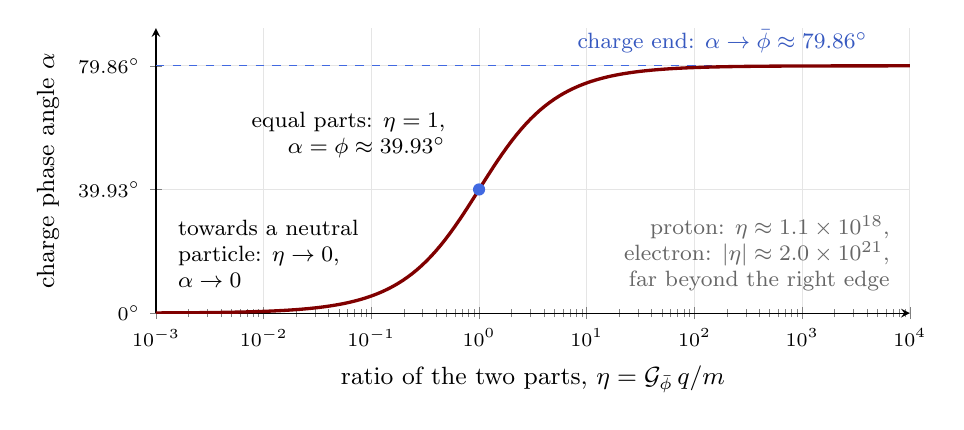
\begin{tikzpicture}
  \begin{axis}[
    width=0.92\textwidth, height=5.2cm,
    xmode=log, xmin=1e-3, xmax=1e4, ymin=0, ymax=92,
    xtick={1e-3,1e-2,1e-1,1,1e1,1e2,1e3,1e4},
    ytick={0,39.93,79.86}, yticklabels={$0^\circ$,$39.93^\circ$,$79.86^\circ$},
    xlabel={ratio of the two parts, $\eta = \mathcal{G}_{\bar{\phi}}\,q/m$},
    ylabel={charge phase angle $\alpha$},
    axis lines=left, grid=major, grid style={gray!20},
    tick label style={font=\scriptsize}, label style={font=\small}]
    \draw[RoyalBlue, dashed] (1e-3,79.86) -- (1e4,79.86);
    \addplot[very thick, Maroon, domain=-3:4, samples=160] ({10^x}, {atan(10^x*0.98438/(1 + 10^x*0.17605))});
    \fill[RoyalBlue] (1,39.93) circle (2.2pt);
    \node[font=\footnotesize, anchor=south east, align=right] at (0.6,47) {equal parts: $\eta = 1$,\\ $\alpha = \phi \approx 39.93^\circ$};
    \node[font=\footnotesize, anchor=south east, text=RoyalBlue!85!black] at (5e3,81) {charge end: $\alpha \to \bar{\phi} \approx 79.86^\circ$};
    \node[font=\footnotesize, anchor=south west, align=left] at (1.3e-3,5) {towards a neutral\\ particle: $\eta \to 0$,\\ $\alpha \to 0$};
    \node[font=\footnotesize, anchor=south east, align=right, text=gray!80!black] at (8e3,4) {proton: $\eta \approx 1.1 \times 10^{18}$,\\ electron: $|\eta| \approx 2.0 \times 10^{21}$,\\ far beyond the right edge};
  \end{axis}
\end{tikzpicture}
\caption[From a ratio to an angle]{From a ratio to an angle (Remark~\ref{rem:charge-phase} with $k = 0$), on a scale of powers of ten. At $\eta = 1$ the two parts are equal and $\alpha$ is half of $\bar{\phi}$. As $\eta$ grows, $\alpha$ climbs towards $\bar{\phi} \approx 79.86^\circ$, the charge end. The proton lies far beyond the right edge of the picture, and so does the electron, on the side flipped by $k\pi$.}
\label{fig:charge-phase}
\end{figure}

\begin{workedexample}[Worked example: the two ends of the triangle]
\emph{A neutral particle.} The neutron has $q = 0$: its cosmic mass is a real number (Remark~\ref{rem:gn-kinds}), and $\eta = 0$. Remark~\ref{rem:charge-phase} gives $\beta = \arctan(0) = 0$, and with $k = 0$ the charge phase angle is $\alpha = 0$, so the mass phase angle is $\phi = \pb = 79.86^\circ$. Remark~\ref{rem:mass-charge-rep} then gives $m = r \cdot \sin(\pb)/\sin(\pb) = r$. For a neutral particle, the cosmic magnitude is simply the mass, and Remark~\ref{rem:identity-triangle} agrees, since $r^2 = m^2 + 0 + 0$.

\emph{A charge without mass.} At the other end, imagine a particle with charge but no mass. Then $m = 0$, so $\sin(\phi) = 0$ in Remark~\ref{rem:mass-charge-rep}, which gives $\phi = 0$ and $\alpha = \pb$. The particle sits entirely on the charge side, and $r = q\Gp$, the size of its charge part. Remark~\ref{rem:charge-phase} agrees in the limit of a very large ratio $\eta$, where $\beta$ approaches $\arctan(0.98438/0.17605) \approx 79.86^\circ$. The two ends are the first two special triangles of Remark~\ref{rem:special-triangles}, a real number and a pure Composer number.

Every real particle lies somewhere between these two ends, and its charge phase angle $\alpha$ tells how far its identity has turned from pure mass towards pure charge (\Cref{fig:charge-phase}). For a negative charge, the triangle flips to the other side of the mass axis; the term $k\pi$ in Remark~\ref{rem:charge-phase} is there to allow for such flips. Measured through the Composer Unit, the ratios $\eta$ of the electron and the proton are enormous, about $2.0 \times 10^{21}$ and $1.1 \times 10^{18}$ in size, the ratios of the two parts found in \Cref{subsec:cu-size}. So Remark~\ref{rem:charge-phase} places both of them within less than a billionth of a billionth of a radian of the charge end: $\alpha$ is extremely close to $\pb$ for the proton, and to $\pb + \pi$ for the electron, whose charge is negative.
\end{workedexample}

Every number on this card is computed at the angle $79.86^\circ$. The next section reads the law in its own plane, and the last one shows why, at this angle, like charges push apart.

%------------------------------------------------
\section{Reading the Law in Its Own Plane}\label{sec:reading-law}\label{sec:which-angle}
%------------------------------------------------

\scene{Paris, 1733}

In 1733 Charles Fran\c{c}ois de Cisternay du Fay, a chemist in charge of the royal garden of plants in Paris, was working through the new experiments on electricity that Stephen Gray had begun in England. He rubbed a glass tube and let it chase a scrap of gold leaf through the air. The leaf flew to the tube, touched it, and was then pushed away, and it kept its distance as long as the tube followed it. Du Fay expected a rubbed lump of copal, a hard resin like amber, to push the leaf away as well. It pulled the leaf towards itself.

From this surprise he drew a rule. In a letter to the Duke of Richmond he wrote that \enquote{there are two distinct electricities, very different from one another,} and he called them vitreous, from glass, and resinous, from resin: \enquote{a body of the vitreous electricity, for example, repels all such as are of the same electricity; and on the contrary, attracts all those of the resinous electricity} \citep{DuFay1733}. In 1747 Benjamin Franklin gave the two kinds the names that are still in use, positive and negative \citep{Franklin1751}, and in 1785 Coulomb measured how the push between two like charges falls off with distance (Chapter~\ref{ch:one-number}).

Du Fay's rule, with Coulomb's strength, is the first fact that the law must meet, and the simplest atom is the place to test it. But first the law must be read.

\subsection{Two Readings of One Product}\label{subsec:reading}

The Cosmic Interaction Law of \Cref{thm:cosmic-law} gives a General Number multiplied by the arrow $\er$. A laboratory, however, measures one ordinary number along $\er$: so many newtons, pulling or pushing. Before the law can be compared with nature, we need a rule that turns the General Number $\mu_a \mu_b$ into one real number.

Chapter~\ref{ch:general-numbers} offers two such rules, both readings on the real axis, which carries mass (Remark~\ref{rem:part-shadow}).
\begin{itemize}
  \item The \emph{shadow} drops the tip of the number straight down onto the real axis, as a lamp overhead would (Definition~\ref{def:shadow}).
  \item The \emph{real part} walks back to the real axis along the Composer axis, the way the number was built: $a$ steps along the real axis, then $b$ steps of the Composer Unit (Definition~\ref{def:gn-parts}).
\end{itemize}

Two neutral masses must pull together, so in both readings a value forward along the mass axis means a pull, and a value backward means a push. For two neutral bodies the product $\mu_a\mu_b = m_a m_b$ is a real number, and both readings give Newton's law exactly. They part as soon as charge enters.

By \Cref{thm:shadow-product}, the shadow counts each of the three terms of the law with the shadow of its own direction: $1$ for gravity, along the mass axis; $\cos\pb$ for the Coupling Force, which carries the Composer Unit; and $\cos 2\pb$ for the term of two charges, which carries the square $\Gp^2$, an arrow of length $|\Gp|^2$ at the angle $2\pb$ (\Cref{thm:powers}). Since $G\,|\Gp| = \sqrt{KG}$ and $G\,|\Gp|^2 = K$,
\[
G\,\Sh(\mu_a\mu_b) = G\,m_a m_b + \sqrt{KG}\,\cos\pb\,(m_a q_b + q_a m_b) + K\cos 2\pb\;q_a q_b .
\]
Read this way, the electric term keeps the share $\cos 2\pb$ of Coulomb's strength, and the Coupling Force acts along the line with the share $\cos\pb$.

The real part needs one more step. The first two terms of the product are already written as a real number and a Composer part, but the third carries $\Gp^2$, an arrow that leans at $2\pb$. Chapter~\ref{ch:general-numbers} supplies its real part: the Rule of the Square (Proposition~\ref{prop:square-rule}) writes the square as $\Gp^2 = 2\,|\Gp|\cos\pb\;\Gp - |\Gp|^2$, with the real part $-|\Gp|^2$. \Cref{fig:square-readings} shows the two readings of this square side by side at $79.86^\circ$: the walk back along the Composer axis lands at $-1$ times the squared length, and the drop straight down at $-0.938$ times it.

\subsection{The Law Read by Its Real Part}\label{subsec:law-read}

\begin{proposition}[Newton and Coulomb in One Law]\label{prop:law-real}
In the relative plane of the Composer Unit, the product of two cosmic masses is
\[
\mu_a\mu_b = \left(m_a m_b - |\Gp|^2\,q_a q_b\right) + \left(m_a q_b + q_a m_b + 2\,|\Gp|\cos\pb\;q_a q_b\right)\Gp ,
\]
and its real part, multiplied by $G$, is
\[
G\,\Re(\mu_a\mu_b) = G\,m_a m_b - K\,q_a q_b .
\]
The Coupling Force has no real part, and the angle $\pb$ appears only in the Composer coordinate.
\end{proposition}

\begin{proof}
This is Proposition~\ref{prop:un-real-product} with $a = m$ and $b = q$: multiply out the two brackets (Proposition~\ref{prop:three-terms}), $\mu_a\mu_b = m_a m_b + (m_a q_b + q_a m_b)\,\Gp + q_a q_b\,\Gp^2$, and replace $\Gp^2$ by the Rule of the Square. The real part is the first bracket, and $G\,|\Gp|^2 = K$ by the size of the Composer Unit (\Cref{subsec:cu-size}).
\end{proof}

\begin{table}[tb]
\myfloatalign
\small
\begin{tabularx}{\textwidth}{@{}X c c@{}}
\toprule
\tableheadline{term of the law} & \tableheadline{shadow} & \tableheadline{real part} \\
\midrule
gravity, $G\,m_a m_b$ & $1$ & $1$ \\
Coupling Force, $\sqrt{KG}\,(m_a q_b + q_a m_b)$ & $\cos\pb$ & $0$ \\
two charges, $K\,q_a q_b$ & $\cos 2\pb$ & $-1$ \\
\midrule
at $79.86^\circ$ & $1$, $0.17605$, $-0.93801$ & $1$, $0$, $-1$ \\
\bottomrule
\end{tabularx}
\caption[Two readings of the law]{Two readings of the law: the factor with which each of its three terms counts along the line between the two bodies. A positive value means a pull, a negative value a push. The real part gives Newton and Coulomb at full strength; the shadow gives Coulomb's law only the share $\cos 2\pb \approx -0.938$ of its strength, and a Coupling Force along the line with the share $\cos\pb \approx 0.176$.}
\label{tab:two-readings}
\end{table}

Read by its real part, one law gives both of the laws of \Cref{subsec:classical-forces}, each with its full constant, and with opposite signs (\Cref{tab:two-readings}). The minus sign is the one that Definitions~\ref{def:newton} and~\ref{def:coulomb} left to the nature of each interaction (\Cref{fig:pull-push}): two masses pull, and the term of two charges, for like charges, counts the other way and pushes. No factor of the angle remains in any force. The Coupling Force of Remark~\ref{rem:three-components} has no real part at all: read in its own plane, it is not a force along the line. It lives, with the angle, in the Composer coordinate of the product (\Cref{fig:square-split}).

It does not live there alone. By \Cref{thm:gn-parts-product}, the Composer coordinate of a product is built from the shadows $\Sh(\mu) = m + |\Gp|\cos\pb\;q$ of the two factors (Definition~\ref{def:shadow}):
\[
m_a q_b + q_a m_b + 2\,|\Gp|\cos\pb\;q_a q_b = \Sh(\mu_a)\,q_b + \Sh(\mu_b)\,q_a .
\]
Beside the Coupling term it holds a share of the term of two charges, $2\,|\Gp|\cos\pb\;q_a q_b$, and for charged particles that share is by far the larger: the Coupling term is $5 \times 10^{-18}$ of it for two protons and $3 \times 10^{-21}$ of it for two electrons. Read like a force, multiplied by $G/r^2$, the Composer part of the product of two charged particles is an arrow about $2\cos\pb \approx 0.352$ times as long as Coulomb's force between them. Only between a neutral body and a charge is the whole Composer coordinate the Coupling term.

\begin{figure}[tb]
\myfloatalign
\begin{tikzpicture}[>=Stealth, every node/.style={font=\footnotesize},
    box/.style={draw, rounded corners=2pt, text width=4.3cm, minimum height=1.25cm, align=center, inner sep=4pt}]
  \node[box, fill=gray!12, text width=7.4cm, minimum height=0.9cm] (t) at (3.3,1.75) {$\mu_a\mu_b = m_a m_b + (m_a q_b + q_a m_b)\,\mathcal{G}_{\bar{\phi}} + q_a q_b\,\mathcal{G}_{\bar{\phi}}^2$};
  \node[box, fill=RoyalBlue!10, draw=RoyalBlue!60] (a) at (0,0) {\textbf{real part}\\ $m_a m_b - |\mathcal{G}_{\bar{\phi}}|^2\,q_a q_b$\\ times $G$: Newton and Coulomb, at full strength};
  \node[box, fill=white, draw=gray!70, densely dashed] (b) at (6.6,0) {\textbf{Composer coordinate}\\ $m_a q_b + q_a m_b + 2\,|\mathcal{G}_{\bar{\phi}}|\cos\bar{\phi}\;q_a q_b$\\ the Coupling Force and the angle};
  \draw[->, thick] (t.south) ++(-0.6,0) -- (a.north);
  \draw[->, thick] (t.south) ++(0.6,0) -- (b.north);
\end{tikzpicture}
\caption[The product splits in two]{The product of two cosmic masses splits in two (Proposition~\ref{prop:law-real}). Its real part is the force along the line: gravity and Coulomb's law, each at full strength. Its Composer coordinate holds the Coupling Force and the angle of the Composer axis, and it is not read as a force. Beside the Coupling Force it also holds a share of the term of two charges, by far the larger part for charged particles (\Cref{subsec:law-read}).}
\label{fig:square-split}
\end{figure}

\subsection{The Hydrogen Test}\label{subsec:test-sign}

Without Du Fay's rule there would be no atoms: the electron of a hydrogen atom is held in place by the pull of the proton. The pull must have the right sign, and it must also have the right size, because the size sets how tightly the electron is bound.

% keep what follows together: break the page here if fewer than 10 lines are left
\keepblock{10}
\begin{workedexample}[Worked example: the hydrogen atom]
In a hydrogen atom the electron and the proton are about $a_0 = 5.29 \times 10^{-11}$ m apart, and their charges are $+e$ and $-e$, with $e = 1.602 \times 10^{-19}$ C.
\begin{itemize}
  \item \emph{Nature.} Coulomb's law gives a pull of size $K e^2/a_0^2$. Step by step: $e^2 \approx 2.566 \times 10^{-38}$ C$^2$; then $K e^2 \approx 8.98755 \times 10^{9} \times 2.566 \times 10^{-38} \approx 2.307 \times 10^{-28}$ N\,m$^2$; and $a_0^2 \approx 2.798 \times 10^{-21}$ m$^2$. Dividing, the pull is about $8.24 \times 10^{-8}$ N.
  \item \emph{The law, read by its real part.} With $q_a q_b = -e^2$, Proposition~\ref{prop:law-real} gives the electric part $-K\,(-e^2)/a_0^2 = +K e^2/a_0^2$: a pull of $8.24 \times 10^{-8}$ N.
  \item \emph{The law, read by its shadow.} The electric term counts with $\cos 2\pb$. At $79.86^\circ$ it is a pull of $0.93801 \times 8.24 \times 10^{-8} \approx 7.73 \times 10^{-8}$ N, only $93.8\%$ of the strength.
  \item \emph{How tightly the electron is held.} In Bohr's model of the atom, the energy needed to free the electron grows with the square of the strength of the pull \citep{Bohr1913}. With the full strength of Coulomb's law it is $13.598$ eV, the measured value \citep{Sansonetti2005}. With $93.8\%$ of the strength it would be $0.93801^2 \times 13.598 \approx 11.96$ eV, short by $1.6$ eV.
\end{itemize}
\end{workedexample}

\emph{A second test: the neutron.} The shadow also keeps the share $\cos\pb$ of the Coupling Force. Between a neutral body of mass $m$ and a charge, that share acts exactly like an electric force on a body of charge
\[
Q = \cos\pb\,\sqrt{G/K}\;m ,
\]
so every neutral body would carry an apparent charge in proportion to its mass. For the neutron, at $79.86^\circ$, $Q \approx 0.17605 \times 8.617 \times 10^{-11}\ \mathrm{C/kg} \times 1.675 \times 10^{-27}\ \mathrm{kg} \approx 1.59 \times 10^{-19}\,e$. The charge of the neutron has been measured, by bending beams of slow neutrons in strong electric fields and by testing the neutrality of a gas, and found to be $(-0.2 \pm 0.8) \times 10^{-21}\,e$ \citep{Baumann1988,Bressi2011,PDG2024}. The shadow misses by about two hundred standard errors. Read by its real part, the Coupling Force is zero, and so is the apparent charge.

\suppressfloats[t]
\begin{figure}[tb]
\myfloatalign
\begin{tikzpicture}[>=Stealth, every node/.style={font=\small},
    proton/.style={draw, circle, fill=RoyalBlue!12, minimum size=0.75cm, inner sep=0pt},
    electron/.style={draw, circle, fill=Maroon!10, minimum size=0.75cm, inner sep=0pt}]
  \def\xa{2.3}
  \def\xb{6.2}
  % nature
  \node[anchor=east, font=\footnotesize, align=right] at (0.95,0) {nature};
  \node[proton] (p1) at (\xa,0) {$+$};
  \node[electron] (e1) at (\xb,0) {$-$};
  \draw[->, very thick, gray!70!black] (p1.east) -- ++(0.8,0);
  \draw[->, very thick, gray!70!black] (e1.west) -- ++(-0.8,0);
  \node[font=\footnotesize, anchor=west] at (6.75,0) {pull, $8.24 \times 10^{-8}$ N};
  % the real part
  \node[anchor=east, font=\footnotesize, align=right] at (0.95,-1.3) {real part};
  \node[proton] (p2) at (\xa,-1.3) {$+$};
  \node[electron] (e2) at (\xb,-1.3) {$-$};
  \draw[->, very thick, RoyalBlue] (p2.east) -- ++(0.8,0);
  \draw[->, very thick, RoyalBlue] (e2.west) -- ++(-0.8,0);
  \node[font=\footnotesize, anchor=west, text=RoyalBlue] at (6.75,-1.3) {pull, $8.24 \times 10^{-8}$ N};
  % the shadow, at 79.86 degrees
  \node[anchor=east, font=\footnotesize, align=right] at (0.95,-2.6) {shadow,\\ $79.86^\circ$};
  \node[proton] (p3) at (\xa,-2.6) {$+$};
  \node[electron] (e3) at (\xb,-2.6) {$-$};
  \draw[->, very thick, gray] (p3.east) -- ++(0.75,0);
  \draw[->, very thick, gray] (e3.west) -- ++(-0.75,0);
  \node[font=\footnotesize, anchor=west, text=gray!80!black] at (6.75,-2.6) {pull, $7.73 \times 10^{-8}$ N};
\end{tikzpicture}
\caption[The hydrogen test]{The hydrogen test (\Cref{subsec:test-sign}). In nature the proton and the electron pull each other together with about $8.24 \times 10^{-8}$ N. Read by its real part, the law gives exactly that pull. Read by its shadow, it gives $\cos 2\bar{\phi}$ times that size: a pull of only $93.8\%$ of the strength.}
\label{fig:hydrogen-test}
\end{figure}

\emph{Result.} The shadow fails the hydrogen test on the strength, and it gives the neutron a charge that measurements rule out. The real part passes all three checks: the sign, the strength and the neutral neutron. It is also the reading that the identity card already uses for a single body, whose mass is its real part, $m = \Re(\mu) = r\cos(\alpha, \phi)$ (Remark~\ref{rem:mass-charge-rep}): the General Sinus projects along the Composer axis, not straight down. From here on, the book reads the law the same way.

Both failures of the shadow have one cause. By Proposition~\ref{prop:gn-parts-readings}, the shadow of a General Number is its real part plus the shadow of its Composer part, $\Sh(z) = \Re(z) + \Sh\bigl(\Com(z)\bigr)$. For the law, the shadow is therefore the real part plus $\cos\pb \approx 0.176$ times the signed length of the Composer part: it lets the Composer coordinate of the product into the force. Between the proton and the electron that coordinate is almost entirely the share of the two charges of \Cref{subsec:law-read}, which takes $2\cos^2\pb \approx 0.062$ of the pull away; between the neutron and a charge it is the Coupling term, which gives the apparent charge.

\begin{definition}[Reading the Law]\label{def:reading}
The force that the Cosmic Interaction Law exerts along $\er$ is the real part of the law,
\[
F = G \cdot \frac{\Re(\mu_a \mu_b)}{r^2} = G \cdot \frac{m_a m_b}{r^2} - K \cdot \frac{q_a q_b}{r^2} ,
\]
a pull when it is positive and a push when it is negative. The Composer coordinate of $\mu_a \mu_b$ is not read as a force.
\end{definition}

\begin{plainwords}
A force is one number along one line, but the law gives a General Number, so it must be brought down to the mass axis. There are two ways: drop it straight down, like a shadow, or walk it back along the leaning axis, the way it was built. Dropping gives the electric force only $93.8\%$ of its strength at our angle, loosens the hydrogen atom by $1.6$ eV, and gives the neutron a charge that nobody has found. Walking gives Coulomb's law exactly, holds the hydrogen atom as tightly as it is held, and leaves the neutron neutral. The book walks.
\end{plainwords}

\subsection{The Law Read from Two Cards}\label{subsec:law-cards}

The identity card of \Cref{sec:identity} and the reading of Definition~\ref{def:reading} meet in one formula. By Euler's formula in a relative plane (\Cref{thm:gn-euler}), a cosmic mass with the card $(r, \alpha, \phi)$ is the exponential $\mu = r\,e^{\alpha\Jp}$, where $\Jp$ is the Turning Unit (Definition~\ref{def:gn-turning-unit}): the magnitude $r$ and the charge phase angle $\alpha$ are the length and the angle of its arrow. Multiplying two cosmic masses multiplies their magnitudes and adds their angles (\Cref{thm:gn-turning}). In this subsection the distance between two bodies is written $d$, the $r$ of Definition~\ref{def:reading}, so that it does not clash with their magnitudes.

\keepblock{16}
\begin{proposition}[The Force from Two Cards]\label{prop:law-cards}
Let two bodies the distance $d$ apart have the identity cards $(r_a, \alpha_a, \phi_a)$ and $(r_b, \alpha_b, \phi_b)$ of Remark~\ref{rem:identity}. Then
\[
\mu_a\mu_b = r_a r_b\,e^{(\alpha_a + \alpha_b)\Jp} ,
\]
and the force of Definition~\ref{def:reading} is
\[
F = G\,\frac{r_a r_b}{d^2}\,\cos(\alpha_a + \alpha_b, \pb - \alpha_a - \alpha_b) = G\,\frac{r_a r_b}{d^2}\cdot\frac{\sin(\pb - \alpha_a - \alpha_b)}{\sin\pb} .
\]
With angles counted modulo $360^\circ$, it is a pull when $\alpha_a + \alpha_b$ lies between $\pb - 180^\circ$ and $\pb$, a push when it lies between $\pb$ and $\pb + 180^\circ$, and zero exactly when $\alpha_a + \alpha_b$ is $\pb$ or $\pb + 180^\circ$, that is, when $G\,m_a m_b = K\,q_a q_b$.
\end{proposition}

\begin{proof}
By \Cref{thm:gn-euler}, every nonzero General Number is $|z|\,e^{\alpha\Jp}$, with $\alpha$ the angle of its arrow. For a cosmic mass $|\mu| = r$, and $\alpha$ is the charge phase angle, because the polar form of \Cref{thm:gn-polar} is the card of Remark~\ref{rem:mass-charge-rep}. The rule $e^{w_1 + w_2} = e^{w_1}e^{w_2}$ gives the product. With $\theta = \alpha_a + \alpha_b$, \Cref{thm:gn-polar} gives the real part of $r_a r_b\,e^{\theta\Jp}$ as $r_a r_b\cos(\theta, \pb - \theta)$, and the definition of the General Sinus gives $\cos(\theta, \pb - \theta) = \sin(\pb - \theta)/\sin\pb$. Multiplied by $G/d^2$, this is the force. Its sign is the sign of $\sin(\pb - \theta)$, which gives the two bands, and it is zero exactly when $\sin(\pb - \theta) = 0$. The same real part is $m_a m_b - |\Gp|^2 q_a q_b$ (Proposition~\ref{prop:law-real}), so the force is zero exactly when $G\,m_a m_b = K\,q_a q_b$.
\end{proof}

Read on the cards, Du Fay's rule needs only the angles. Two neutral bodies have $\alpha = 0$: their angles add up to $0^\circ$, and they pull. A proton lies within $10^{-16}$ degree of the angle $\pb$, and an electron within as little of $\pb + 180^\circ$ (\Cref{subsec:id-phase}). Two protons, or two electrons, add up to about $2\pb = 159.72^\circ$ and push; a proton and an electron add up to about $339.72^\circ$ and pull. These are the angles of \Cref{fig:line-and-plane}, now for every pair of bodies. A pair neither pulls nor pushes when its angles add up to $\pb$, as for two positive bodies whose two parts are equal, each on the ray $\alpha = \pb/2 \approx 39.93^\circ$ (\Cref{fig:triangles-to-scale}(b)), or to $\pb + 180^\circ$, as for two such bodies with negative charges. The proposition is a reading of the law, not a new fit: the force is still $G\,m_a m_b - K\,q_a q_b$ over $d^2$, and at another angle the cards would change and give the same force.

\keepblock{10}
\begin{workedexample}[Worked example: three pairs, read from their cards]
Put each pair $1$ m apart.
\begin{itemize}
  \item \emph{Two protons.} Each card has $r \approx e\,|\Gp| \approx 1.85921 \times 10^{-9}$ kg, and the angles add up to $2\pb \approx 159.72^\circ$, less about $10^{-16}$ degree, so the factor $\sin(\pb - \alpha_a - \alpha_b)/\sin\pb$ is $-1$ to many digits. The force is $-G\,(1.85921 \times 10^{-9})^2 \approx -2.307 \times 10^{-28}$ N: a push of Coulomb's strength, since $G\,|\Gp|^2 = K$.
  \item \emph{A proton and an electron.} The angles add up to $339.72^\circ$, the factor is $+1$, and the same product of magnitudes gives a pull of $2.307 \times 10^{-28}$ N.
  \item \emph{A neutron and a proton.} The neutron has $r = m_n$ and $\alpha = 0$, so the sum is the angle of the proton, short of $\pb$ by $\delta \approx 5.07 \times 10^{-17}$ degree. The factor is $\sin\delta/\sin\pb$, and $r_p\sin\delta/\sin\pb = m_p$ by Remark~\ref{rem:mass-charge-rep}, so the force is $G\,m_n m_p \approx 1.87 \times 10^{-64}$ N: gravity alone.
\end{itemize}
\end{workedexample}

%------------------------------------------------
\section{Why Like Charges Push Apart}\label{sec:why-mirror}
%------------------------------------------------

Du Fay found the rule, and Coulomb measured it, but neither said why: the classical laws take the sign from experiment and write it in by hand (\Cref{fig:pull-push}).

Physics has since found a deeper reason, in a different kind of theory. In quantum field theory a force is carried by a particle that the two bodies exchange, and the sign of the force between two like sources follows from the spin of that particle: the exchange of a particle of spin one, such as the photon, pushes like charges apart, while the exchange of a particle of spin zero or spin two, the spin expected of the graviton, pulls like sources together \citep{Zee2010}. The Cosmic Interaction Law is a classical law between two bodies, and it gives the same fact a reason of another kind, a geometric one.

\begin{figure}[tb]
\myfloatalign
\begin{tikzpicture}[>=Stealth, every node/.style={font=\footnotesize}]
  % (a) on a line: all products lie on the mass axis (drawn side by side)
  \node[anchor=west, font=\small] at (-4.6,2.05) {(a) on a line: a real unit $\lambda$};
  \draw[gray] (-4.6,0) -- (4.6,0);
  \node[gray, anchor=north west] at (-4.6,-0.05) {push};
  \node[gray, anchor=north east] at (4.6,-0.05) {pull};
  \node[gray, anchor=north] at (0,-0.08) {mass axis};
  \draw[gray!60, densely dotted] (0,0) -- (0,1.62);
  \fill (0,0) circle (1.3pt);
  \draw[->, very thick, gray!70!black] (0,1.45) -- (2.2,1.45) node[right] {two masses: pull};
  \draw[->, very thick, RoyalBlue] (0,0.95) -- (2.2,0.95) node[right] {like charges: pull};
  \draw[->, very thick, RoyalBlue, densely dashed] (0,0.45) -- (-2.2,0.45) node[left] {unlike charges: push};
  % (b) in the plane: the walk back along the Composer axis at the mirror root
  \begin{scope}[shift={(0,-3.8)}]
    \def\L{3.2}
    \node[anchor=west, font=\small] at (-4.6,2.55) {(b) in the plane: the Composer Unit at $79.86^\circ$};
    \draw[gray] (-4.6,0) -- (4.6,0);
    \node[gray, anchor=north west] at (-4.6,-0.05) {push};
    \node[gray, anchor=north east] at (4.6,-0.05) {pull};
    \draw[gray!50, densely dotted] (0,0) -- (79.86:1.7) node[right, font=\scriptsize, text=gray!80!black] {Composer axis};
    % like charges: the square, reached by the walk -L then 0.35210 L along the axis
    \draw[->, very thick, gray!70!black] (0,0) -- (-\L,0);
    \draw[->, thick, RoyalBlue] (-\L,0) -- ($(-\L,0)+(79.86:{0.35210*\L})$);
    \draw[->, very thick, RoyalBlue!50] (0,0) -- (159.72:\L);
    \node[RoyalBlue!85!black, anchor=south] at ($(159.72:\L)+(0.15,0.06)$) {like charges, $159.72^\circ$};
    \node[anchor=north, font=\scriptsize] at (-1.6,-0.08) {real part $-|\mathcal{G}_{\bar{\phi}}|^2$: push};
    % unlike charges: minus the square, reached by +L then -0.35210 L along the axis
    \draw[->, very thick, gray!70!black] (0,0) -- (\L,0);
    \draw[->, thick, RoyalBlue] (\L,0) -- ($(\L,0)+(259.86:{0.35210*\L})$);
    \draw[->, very thick, RoyalBlue!50, densely dashed] (0,0) -- (339.72:\L);
    \node[RoyalBlue!85!black, anchor=north] at ($(339.72:\L)+(0.1,-0.08)$) {unlike charges, $339.72^\circ$};
    \node[anchor=south, font=\scriptsize] at (1.6,0.06) {real part $+|\mathcal{G}_{\bar{\phi}}|^2$: pull};
    \fill (0,0) circle (1.3pt);
  \end{scope}
\end{tikzpicture}
\caption[On a line and in the plane]{On a line and in the plane (\Cref{subsec:why-line,subsec:why-doubles}). The products of the law for pairs of bodies, read along the mass axis: to the right is a pull, to the left a push. (a) With a real number in the place of the Composer Unit, every product lies on the mass axis (drawn side by side): like charges pull as masses do, and unlike charges push, the opposite of nature. (b) With the Composer Unit at $79.86^\circ$, the product of two like charge parts leans at $159.72^\circ$. Walked back along the Composer axis, it reaches the mass axis at $-|\mathcal{G}_{\bar{\phi}}|^2$: a push of Coulomb's full strength. For unlike charges the product turns half a turn, to $339.72^\circ$, and the walk reaches $+|\mathcal{G}_{\bar{\phi}}|^2$: a pull. The lengths are not to scale.}
\label{fig:line-and-plane}
\end{figure}

\subsection{On a Line, Like Charges Would Pull}\label{subsec:why-line}

Suppose that mass and charge had been put into one ordinary number, $\mu = m + \lambda q$, with a real number $\lambda$, in kilograms per coulomb, in the place of the Composer Unit. The product of two such numbers multiplies out exactly as in \Cref{fig:product-area}:
\[
\mu_a \mu_b = m_a m_b + \lambda\,(m_a q_b + q_a m_b) + \lambda^2\,q_a q_b .
\]
Whatever the number $\lambda$, positive or negative, its square is positive (Remark~\ref{rem:line-forward}). For two like charges $q_a q_b$ is positive too, so the last term has the sign of the first: one law built on this product would pull two like charges together exactly as it pulls two masses, and it would push a proton away from an electron. The choice $\lambda^2 = K/G$ would give the electric term the strength of Coulomb's law, but no choice of $\lambda$ can give it the sign. Turning the whole law around does not help either, since two masses would then push apart.

A real number in the place of the Composer Unit makes the relative plane a line, no plane (Remark~\ref{rem:line-no-plane}): the two parts of a cosmic mass simply add, and charge acts as extra mass. On a line, one product of cosmic masses can carry the sign of gravity or the sign of electricity, but never both (\Cref{fig:line-and-plane}(a)). To carry both, the law needs a unit whose square points the other way, back along the mass axis. The Composer Unit, leaning at $79.86^\circ$, is such a unit.

\subsection{In the Plane, Like Charges Push}\label{subsec:why-doubles}

The Rule of the Square (Proposition~\ref{prop:square-rule}) gives the square of the Composer Unit the real part $-|\Gp|^2$, a negative number, and the law read by its real part turns it into the electric term of Proposition~\ref{prop:law-real}. Step by step:
\begin{enumerate}
  \item By Proposition~\ref{prop:law-real}, the electric part of the force along $\er$ is $-K\,q_a q_b/r^2$, where a negative value is a push (Definition~\ref{def:reading}).
  \item For like charges $q_a q_b$ is positive, so the electric part is a push; for unlike charges it is negative, and the same expression is a pull.
  \item The constant is Coulomb's constant $K$ itself, so the push and the pull have the full strength of Coulomb's law.
\end{enumerate}
One fact gives both halves of Du Fay's rule, at Coulomb's strength (\Cref{fig:line-and-plane}(b)): the square of the Composer Unit points back along the mass axis. \Cref{prop:law-cards} reads the same rule off the cards of any two bodies.

% keep what follows together: break the page here if fewer than 9 lines are left
\keepblock{9}
\begin{plainwords}
Picture the mass axis as a floor. The term of two masses is a stick lying flat on the floor and pointing forward; the term of two charges is a stick that leans at $159.72^\circ$, twice the angle of the Composer axis. Walk its tip back to the floor along the leaning axis: the walk lands behind the starting point, at minus the squared length, and behind means a push. Make one of the charges negative, and the walk lands in front: a pull. On a line the stick of two charges would lie flat and point forward, and like charges would pull as masses do.
\end{plainwords}

\begin{workedexample}[Worked example: two protons]
Two protons one metre apart push each other apart, in nature, with $K e^2 \approx 2.31 \times 10^{-28}$ N. Read by its real part, the law gives $-K e^2/r^2 \approx -2.31 \times 10^{-28}$ N: a negative number, a push, at Coulomb's full strength. The shadow, the drop straight down, gives $\cos 159.72^\circ \approx -0.93801$ times as much, $-2.16 \times 10^{-28}$ N: a push too, but at $93.8\%$ of the strength, the shortfall that the hydrogen test of \Cref{subsec:test-sign} detects.
\end{workedexample}

\subsection{Why the Angle Is 79.86 Degrees}\label{subsec:which-root}

Read by its real part, the force between two bodies contains the size of the Composer Unit, through $G\,|\Gp|^2 = K$, but not its angle. The real part of a product has no angle in it (Proposition~\ref{prop:un-real-product}); the angle lives in the Composer coordinate, with the Coupling term, and in the corner of every particle triangle, $\alpha + \phi = \pb$ (Remark~\ref{rem:identity}). So no measured force fixes the angle. The size of the Composer Unit gives it, as the mirror root of \Cref{subsec:cu-angle}, $79.86^\circ$, and the book holds it there from this point to the end.

The reason for this angle is the one given in \Cref{subsec:cu-angle}: at $79.86^\circ$ the push of like charges can be seen in the plane itself. The square of the Composer Unit leans at $159.72^\circ$, inside the backward band of \Cref{thm:square-band} (Corollary~\ref{cor:roots-band}), so the arrow of two like charges points back along the mass axis, against the arrow of two masses. The two readings of the law then agree in sign: the real part of the square is $-|\Gp|^2$, and its shadow, $|\Gp|^2\cos 159.72^\circ \approx -0.938\,|\Gp|^2$, falls behind the origin too (\Cref{fig:square-readings}). This is a choice of coherence, not a fit to data, and no number measured in this book depends on it. \Cref{tab:two-roots} gathers the numbers of the Composer Unit at this angle, which the next three chapters use.

\begin{table}[tb]
\myfloatalign
\begin{tabularx}{\textwidth}{@{}>{\raggedright\arraybackslash}X c@{}}
\toprule
\tableheadline{number} & \tableheadline{value} \\
\midrule
angle $\pb$ of the Composer Unit & $79.86^\circ$ \\
$\cos\pb$; $\sin\pb$ & $0.17605$; $0.98438$ \\
length $|\Gp| = \sqrt{K/G}$ & $1.16043 \times 10^{10}$ kg/C \\
angle $2\pb$ of $\Gp^2$ & $159.72^\circ$ \\
$\cos 2\pb$; $\sin 2\pb$ & $-0.93801$; $0.34660$ \\
real part of $\Gp^2$, over $|\Gp|^2$ & $-1$ \\
Composer coordinate of $\Gp^2$, over $|\Gp|$: $2\cos\pb$ & $0.35210$ \\
shadow of $\Gp^2$, over $|\Gp|^2$: $\cos 2\pb$ & $-0.93801$ \\
corner of a particle triangle whose two parts have the same sign, $180^\circ - \pb$ & $100.14^\circ$ \\
\bottomrule
\end{tabularx}
\caption[The Composer Unit in numbers]{The Composer Unit of our universe in numbers (\Cref{subsec:cu-size,subsec:which-root}). Chapters~\ref{ch:standard-model} to~\ref{ch:unified} use these numbers.}
\label{tab:two-roots}
\end{table}

%------------------------------------------------
\section*{Looking Back, and Ahead}\phantomsection\label{sec:interaction-close}
%------------------------------------------------

Faraday looked for a link between gravity and electricity, and the cosmic mass offers one, though not the kind he looked for. It is not a new force. Read in its own plane, the law has no part along the line between the mass of one body and the charge of the other: the Coupling Force of Remark~\ref{rem:three-components} lives in the Composer coordinate, beside, for charged particles, a far larger share of the term of two charges, and Faraday's needle, which stayed at zero, is not asked to move. The link is the law itself. One number holds the mass and the charge of a body, one product of two such numbers holds gravity and electricity, and the minus sign that pushes like charges apart, which Du Fay found and Coulomb measured, comes from the plane: the square of the Composer Unit has a negative real part (Proposition~\ref{prop:square-rule}). Read on the identity cards, the same law multiplies the magnitudes of the two bodies and adds their angles (\Cref{prop:law-cards}). Read this way, the law says what Newton and Coulomb say, and no more; its test is that it agrees with them, which it does exactly.

The angle of the Composer axis is held at $79.86^\circ$, where the plane itself shows the push of like charges (\Cref{subsec:which-root}). With the angle fixed, every body of ordinary matter has one triangle, whose corner between the mass side and the charge side is set by the angle alone. The next chapter starts there. It draws all the triangles of one size at once, finds that they line up on one ellipse, and builds from the ellipses a frame in which the electron, the proton, the neutron, the atoms, the ions and the nuclei all have their place: the Cosmic Mass Standard Model of Chapter~\ref{ch:standard-model}.
